\chapter{Results and Conclusions}
\label{ch:res}

In this chapter we use the forward model to generate data and explain how we characterise posterior distributions.
We compare to a ground truth and draw conclusion about how inforamtive the data is.
In doing so we set up a Bayesian framework and guide the reader through the process of prior modelling.
We then present results and compare the tensor train approximation of the posterior with samples from posterior distribution the generated by Markov chain Monte-Carlo (MCMC) methods.
All programming and analysis is done in python on a MacBook Pro from 2019 with 2.4 Ghz quadcore intel core i5 processor.

\section{Simulate Data and ground truth}
We take a ground truth ozone profile generated from some data \cite{MLSdata} of the microwave limb sounder on the aura satellite in the Antarctic region with a peak in high altitude to show that the data is uninformative in those regions, see Fig. \ref{fig:O3Samp}.

From \cite{MLSdata} we get ozone volume mixing ratios and pressure tuples.
We connect pressure and height values recursively with the hydrostatic equilibrium equation
\begin{align}
	\frac{\text{d}p}{p} = \frac{- g M}{R^* T} \text{d} h \, ,
\end{align}
with the acceleration due to gravity
\begin{align}
	g = g_0 \Bigg( \frac{r_0}{r_0 + h} \Bigg) \, ,
\end{align}
where the polar radius pf the earth is $r_0 \approx 6356 \, \text{km}$, the gravitation at sea level is $g_0 \approx 9.81 \text{m}/\text{s}^2$, $R^* = 8.31432 \times 10^{-3} \text{Nm} / \text{kmol} / \text{K}$ and the mean molecular weight of the air is set to $M = 28.97 \text{kg/kmol}$ \cite{atmosphere1976us}.
This holds up to a geometric height of $86$km, where ignore a $0.04\%$ change in $M$ from $80$km to $86$km in geometric altitude.

Following \cite{atmosphere1976us} we can form a temperature function
\begin{align}
	T(h) = \begin{cases*}
		T_0, & \text{$h = 0$}\\
		T_0 + a_0 h , & \text{$0 \leq h < h_{1}$}\\
		T_0 + a_0 h_{1}, & \text{$h_{1} \leq  h < h_{2}$}\\
		T_0 + a_0 h_{1} + a_1 (h   - h_2),  & \text{$h_{2} \leq h < h_{3}$}\\
		T_0 + a_0 h_{1} + a_1 (h_{3} - h_{2}) + a_2 (h   - h_3), & \text{$h_{3} \leq h < h_{4}$}\\
		T_0 + a_0 h_{1} + a_1 (h_{3} - h_{2}) + a_2 (h_{4} - h_{3}), & \text{$h_{4} \leq h < h_{5}$}\\
		T_0 + a_0 h_{1} + a_1 (h_{3} - h_{2}) + a_2 (h_{4} - h_{3}) + a_3 (h   - h_{5}), & \text{$h_{5} \leq h < h_{6}$}\\
		T_0 + a_0 h_{1} + a_1 (h_{3} - h_{2}) + a_2 (h_{4} - h_{3}) + a_3 (h_{6} - h_{5}) + a_4 (h - h_{6}), & \text{$h_{6} \leq h \lesssim 86$}
	\end{cases*} 
	\label{eq:tempFunc}
\end{align}
with values
\begin{tabular}{ |c||c|c|  }
	\hline
	subscript $i$ & geometric height $h_i$ in km&gradient $a_i$\\
	\hhline{|=||=|=|}
	0& 0 & -6.5\\
	1& 11 & 0\\
	2& 20.1& 1\\
	3& 32.2& 2.8\\
	4& 47.4& 0\\
	5& 51.4& -2.8\\
	6& 71.8& -2\\
	\hline
\end{tabular}
as in \cite{atmosphere1976us}, we plot the ground truth temperature in Fig. \ref{fig:PriorTemp}.
\textcolor{red}{isothermal layers we are able to change the thickenss but we accept that they are is thermeonal we do not model 0.}
Then we can compute a data vector $\bm{y}$, with $m = 42$ measurements according to the radiative transfer equation \ref{eq:RTE}, determined by the satellite pointing accuracy of $150$arcsec as requested in \cite{CubeSatInternal}, within an atmosphere $h_{L,0}=7$km and $h_{L,n} = 83.3$km with $n = 45$ layers.
The height values $h_{L,i}$ for each layer $i = 0,\dots, n$ are defined by the given ozone profile and its pressure values.
We target thermal radiation at a wave number $\nu = 7.86\text{cm}^{-1}$, equal to a frequency of roughly $235$GHz, where we assume that ozone is the only emitter and calculate the absorption constant $k(\nu,T)$ according to the \textit{HITRAN} database \cite{gordon2022hitran2020} for the isotopologue $\prescript{16}{}{\text{O}}_3$ with the AFGL Code 666.
Lastly we add normally distributed $\bm{\nu} \sim \mathcal{N}(0,\gamma^{-1} \bm{I})$ noise so that we have a voltage Signal-to-Noise (SNR) of $60$, similar to THz module on the MLS aura satellite \cite{pickett2006snr}.

To the pressure values in between $h_{L,0}=7$km and $h_{L,n} = 83.3$km we can fit an exponential function
\begin{align}
	p(h) =
	\exp{ \{ -b \,  (h - h_{0} ) \} } \,  p_0 \, ,
	\label{eq:pressFunc}
\end{align}
with the gradient $b$ and the tuple $(p_0,h_{0})$, which will serve as our ground truth pressure function as plotted in Fig. \ref{fig:PriorPress}.


\section{Set up the Bayesian framework}
\label{sec:BayModel}

Given the data and the forward model we set up our Bayesian framework.
In doing so we first draw a directed acyclic graph (DAG) to visualise the measurement and modelling process and determine correlations within some prior distribution are already determined.
Then we define prior distribution over all parameters, which then leads us to the posterior distributions including a likelihood.

We draw a DAG for the measurement and modelling process, where put the hyper-parameters $\gamma, \delta, h_0, p_0, b, \bm{h}, \bm{T}_0, \bm{a}$ on the top and parameters $\bm{x}, \bm{p}/\bm{T}$ further down.
These parameters go into the forward model $\bm{A}_{NL}$ and generate some noisy data $\bm{y}$, where the noise is described through the hyper-parameter $\gamma$, from space of all measurable noise free data $\bm{\Omega}$.

The hyper-parameter related to the ozone is $\delta$, describing the smoothness of the ozone profile $\bm{x}$, and determines the distribution over the ozone profiles, which we set to be a normal distribution, see section \ref{sec:bayes}, as we like to deal with a linear-Gaussian inverse problem.

Since we can describe pressure $\bm{p}$ and temperature $\bm{T}$ through the functions in Eq. \ref{eq:tempFunc} and \ref{eq:pressFunc} we include their function parameters as hyper-parameters in Fig. \ref{fig:DAGComplete}.
Then we can already see the correlation between pressure and temperature since it goes like $\bm{p}/ \bm{T}$ into the forward model.

\textcolor{red}{say that we treat ozone and pressure and temperature separately}
\begin{figure}[thb!]
	\centering
	\begin{tikzpicture}
		\node[roundnode2] at (-4.5,6.5) (Q)     {$\bm{Q}$};
		\node[roundnode2] at (-3,5) (x)     {$\bm{x}$};
		\node[align=center] at (-1,4) (A)    {$\bm{A}(\bm{x},\bm{p},\bm{T})$};
		\node[roundnode2] at (-1,2.5) (u)    {$\bm{\Omega}$};
		\node[rectnode] at (-1,1) (y)    {$\bm{y}$};
		\node[roundnode2] at (-2.5,2.5) (e)    {$\bm{\eta}$};
		\node[roundnode2] at (-6.25,6.5) (S)    {$\bm{\Sigma}$};
		\node[roundnode2] at (-7.75,8) (s)    {$\gamma$};
		\node[roundnode2] at (-6,8) (d)    {$\delta$};
		\node[roundnode2] at (3,6.5) (t)     {$\bm{T}$};
		\node[roundnode2] at (-1,6.5) (p)     {$\bm{p}$};
		\node[roundnode2] at (1,5) (pt)     {$\bm{p}/\bm{T}$};
		\node[roundnode2] at (0,8) (b1)    {$b$};
		%\node[roundnode2] at (1,8) (b2)    {$b_2$};
		\node[roundnode2] at (-2,8) (h1)    {$h_{0}$};
		\node[roundnode2] at (-1,8) (p0)    {$p_0$};
		\node[roundnode2] at (2.25,8) (ht)    {$\bm{h}$};
		\node[roundnode2] at (3.25,8) (ct)    {$T_0$};
		\node[roundnode2] at (4.25,8) (at)    {$\bm{a}$};
		
		%Lines
		\draw[->, very thick] (S.south east) -- (e.north west);
		\draw[->, mydotted, very thick] (s.south east) -- (S.north west);
		\draw[->, very thick] (u.south) -- (y.north);
		\draw[->, mydotted, very thick] (A.south) -- (u.north);
		\draw[->, mydotted,  very thick] (x.south east) -- (A.west);
		\draw[->, mydotted, very thick] (p.south east) -- (pt.north west);
		\draw[->, mydotted, very thick] (t.south west) -- (pt.north east);
		\draw[->, mydotted, very thick] (pt.south west) -- (A.east);
		\draw[->, mydotted, very thick] (h1.south) -- (p.north west);
		\draw[->, mydotted, very thick] (p0.south) -- (p.north);
		\draw[->, mydotted, very thick] (b1.south) -- (p.north east); 
		%\draw[->, very thick] (b2.south) -- (p.east); 
		\draw[->, mydotted, very thick] (d.south east) -- (Q.north west); 
		\draw[->, mydotted, very thick] (e.south east) -- (y.west); 
		
		\draw[->, very thick] (Q.south east) -- (x.north west); 
		\draw[->, mydotted, very thick] (ht.south) -- (t.north west);
		\draw[->, mydotted, very thick] (ct.south) -- (t.north);
		\draw[->, mydotted, very thick] (at.south) -- (t.north east);
		%\node[align=center] at (0.25,3.95) (f3) {$\approx \bm{M A}_L$};
	\end{tikzpicture} 
\caption[Complete directed acyclic graph of the forward model.]{Complete directed acyclic graph of the forward model. The hyper-parameters at the top deterministically (dotted line) describe the parameters ($\bm{p}/\bm{T}$) or the noise covariance $\bm{\Sigma} = \gamma^{-1} \bm{I}$ of the random (solid line) noise $\bm{\eta} \sim \mathcal{N}(0,\gamma^{-1} \bm{I} ) $ and precision matrix $\bm{Q} = \delta \bm{L}$ of the distribution of $\bm{x}\sim \mathcal{N}(0,\delta \bm{L}) $, where $\bm{L}$ is a graph Laplacian as in Eq. \ref{eq:GLapl}. We can group the noise precision $\gamma$  and the smoothness parameter $\delta$ to define the marginal posterior over those hyper-parameters and then condition on them for the conditional posterior distribution,for further details see Fig. \ref{fig:DAGO3}. In this whole process where we condition on the pressure $\bm{p}$ and temperature $\bm{T}$, which we retrieve separately, see Fig. \ref{fig:DAGPT}. The hyper-parameters $h_0,p_0,b$ deterministically describe the pressure function in Eq. \ref{eq:pressFunc}, note that we only need three parameters here since $h_0< h_{L,0}$ and $\bm{h}= \{ h_1, h_2,h_3,h_4,h_5,h_6\}$, $\bm{a} = \{ a_0, a_1, a_2,a_3,a_4\}$ and $T_0$ determine the temperature function.
The parameters $\bm{x}$ and $\bm{p}/ \bm{T}$ determine the space of all measurable noise free data $\bm{\Omega}$ through the forward model $\bm{A}(\bm{x},\bm{p},\bm{T})$ from which we randomly observe data set plus some random noise.}
\label{fig:DAGComplete}
\end{figure}


\begin{align}
	\begin{split}
		\pi(h_1,p_0,b_1,b_2,\bm{h_T},\bm{c_T},\bm{a_T} | \bm{y}, \gamma, \bm{x}) \propto  \exp\Bigl\{ & -\frac{\gamma}{2} \left\Vert \bm{y}- \bm{A} \frac{\bm{p}}{\bm{T}}  \right\Vert^2 \\ &+ \ln{\pi(h_1,p_0,b_1,b_2,\bm{h_T},\bm{c_T},\bm{a_T}) + c \Bigr\}  }
	\end{split} \, ,
\end{align}


Ideally we like to determine the joint posterior
\begin{align}
	\pi(h_1,p_0,b_1,b_2,\bm{h_T},\bm{c_T},\bm{a_T},\delta, \gamma, \bm{x}| \bm{y}) 
\end{align}
but this is computaional not feasible

with normally distributed likelihood function.
\subsection{Prior Modelling}
To complete the Bayesian framework we have define prior distribution for the hyper-parameters and parameters.
Ideally we define the prior distributions as uninformative as possible within functional dependencies and valid physical properties.
In this section we describe how we find the priors and what the priors can already tell us about the results.
We summarise all prior distributions in Tab. \ref{tab:priors} and plot the priors for the hyper-parameters in Fig. \ref{fig:MargPostHistTT} and \ref{fig:PostHistTT0}  to \ref{fig:PostHistTT4} as a dotted black line and for the parameters in Fig. \ref{fig:O3Prior} to \ref{fig:PriorPress}.

\begin{table}
	\centering
	\begin{tabular}{ |c||c|c|c|c|   }
		\hline
		& &\multicolumn{2}{|c|}{TT bounds}&\\
		\hline
		model parameters& priors&\makecell{lower}& \makecell{upper\\
		}&Context\\
		\hhline{|=||=|=|=|=|}
		$\gamma$ & $\mathcal{T}(1,10^{-10})$ &$5 \, 10^{-8}$ &$4.5 \, 10^{-7}$& $\bm{y}$\\ \hline
		$\delta$ &$\mathcal{T}(1,10^{-10})$ & -&-& $\bm{x}$\\ \hline
		$\lambda$ &- & 500&7000& $\bm{x}$\\ \hline
		$\bm{x}$ &$\mathcal{N}(0,\delta \bm{L})$ & -&-& $\bm{x}$\\ \hhline{|=||=|=|=|=|}
		%$\gamma$ & $\mathcal{N}(2.58e-9,2.58e-11)$ &2.45e-9&2.7e-9 &$\bm{x}$\\
		%$\delta_0$ &  $\mathcal{N}(0.8e-4,0.75e-5)$& 4e-5 & 1.1e-4&$\bm{x}$\\
		%$a_0$ &  $\mathcal{T}(3,1e6)$& 1e-15&1e-5&$\bm{x}$\\ \hline
		%$h_0$ &  $\mathcal{N}(31.35,1)$&27 &35&$\bm{x}$\\ \hline
		$h_0$ &  $\mathcal{N}(5.5,0.5)$& 4.76&5.74&$\bm{p/T}$\\ \hline
		$p_0$ &  $\mathcal{N}(500,6)$&479 &519&$\bm{p/T}$\\ \hline
		$b$ &  $\mathcal{N}(0.167,7\,10^{-4})$& 0.165& 0.170 &$\bm{p/T}$\\ \hline
		%$b_2$ & $\mathcal{N}(0.13,0.067)$& 0&0.32&$\bm{p/T}$\\ \hline
		$h_{1}$ &  $\mathcal{N}(11,0.1)$&10.6 &11.3&$\bm{p/T}$\\ \hline
		$h_{2}$ &  $\mathcal{N}(20.1,0.9)$&16.7 &22.8&$\bm{p/T}$\\ \hline
		$h_{3}$ &  $\mathcal{N}(32.3,3)$&23.8&43.6&$\bm{p/T}$\\ \hline
		$h_{4}$ &  $\mathcal{N}(47.4,0.5)$&45.5 &49.3&$\bm{p/T}$\\ \hline
		$h_{5}$ &  $\mathcal{N}(51.4,0.5)$&49.5 &53.3&$\bm{p/T}$\\ \hline
		$h_{6}$ &  $\mathcal{N}(71.8,3)$&60.6 &83.1&$\bm{p/T}$\\ \hline
		$a_{0}$ &  $\mathcal{N}(-6.5,0.01)$&-6.54 &-6.46&$\bm{p/T}$\\ \hline
		$a_{1}$ &  $\mathcal{N}(1,0.01)$&0.96 &1.04&$\bm{p/T}$\\ \hline
		$a_{2}$ &  $\mathcal{N}(2.8,0.1)$&2.43 &3.18&$\bm{p/T}$\\ \hline
		$a_{3}$ &  $\mathcal{N}(-2.8,0.1)$&-3.18 &-2.43&$\bm{p/T}$\\ \hline
		$a_{4}$ & $\mathcal{N}(-2,0.01)$ &-2.04 &-1.96&$\bm{p/T}$\\ \hline
		$T_{0}$ &  $\mathcal{N}(288.15,2)$& 281.8 &294.5&$\bm{p/T}$\\
		\hline
	\end{tabular}
	\caption{Gaussian $\mathcal{N}(\mu,\sigma)$ and gamma distribution $\mathcal{T}(\alpha = \text{scale}, \beta = \text{rate})$
		Bounds for t and p 2.8 times the variance around the mean
		round pressure approx and  test if would work with previous gamma prior or fix gamma prior with set values}
	\label{tab:priors}
\end{table}

\subsubsection{Ozone}
The priors for $\gamma \sim \mathcal{T}(1,10^{-10}) $ and $\delta \sim \mathcal{T}(1,10^{-10})$ are gamma distribution, with parameters chosen so that the distributions are relatively uninformative, see black line in Fig. \ref{fig:MargPostHistTT}.
another reason to choose a gamma distribution is that then the marginal posterior for $\pi(\gamma|\delta,\bm{y})$ is gamma distribution as well and easy to sample from, conjugate prior.

The hyper-parameter delta is defining a prior distribution for ozone $\bm{x} \sim \mathcal{N}(0,\delta \bm{L})$, with 
\begin{align}
	\delta \bm{L} =
	\delta
	\begin{bmatrix}
		2 & -1 & & &  \\
		-1 & 2 & -1 & &   \\
		& \ddots & \ddots & \ddots &\\ 
		& & -1 & 2 & -1  \\
		& & & -1 & 2 
	\end{bmatrix} 
\label{eq:GLapl} 
\end{align}
which is graph Laplacian with Dirichlet boundary conditions \cite{wang2015trend}.
We plot the prior distribution of ozone in Fig. \ref{fig:O3Prior} and see that it is quite uninformative, due to the scale we can  not really see the true Ozone profile and refer to Fig. \ref{fig:O3Samp} or Fig. \ref{fig:O3SolplsReg} for better look at the true ozone profile.
\begin{figure}[ht!]
	\centering
	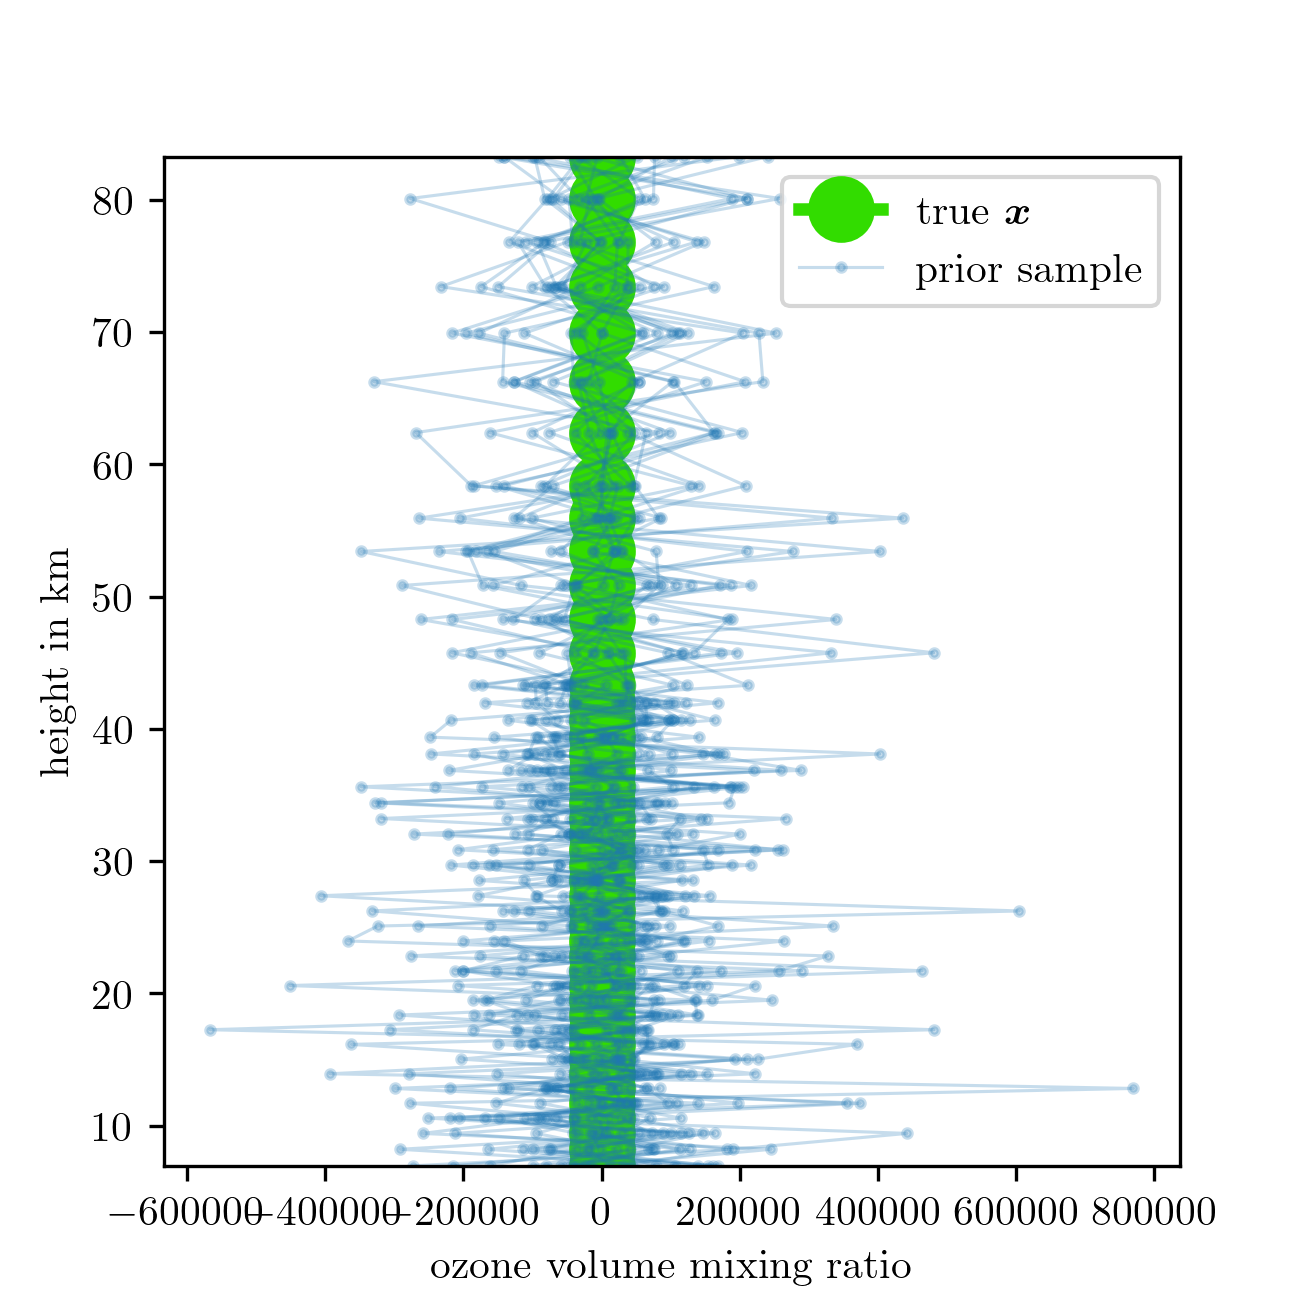
\includegraphics{OzonePrior.png}
	\caption[Samples from ozone prior distribution.]{We draw samples from ozone prior distribution $\bm{x} \sim \mathcal{N}(0,\delta \bm{L})$ after generating a sample from the hyper-prior distribution $\delta \sim \mathcal{T}(1,10^{-10})$. Note that since the spread/variance of prior samples is very large compared to the ozone volume mixing ratios, the ozone profile appears to be constant, which it is not, as seen e.g. in Fig. \ref{fig:O3Samp}.}
	\label{fig:O3Prior}
\end{figure}

\subsubsection{Pressure over temperature}
Next we define the normal hyper-priors for the temperature and pressure hyper-parameters as in table \ref{tab:priors}, which lead to temperature and pressure prior samples see Fig. \ref{fig:PriorTemp} and \ref{fig:PriorPress}.
When plotting the prior samples as $\bm{p} / \bm{T}$ in Fig. \ref{fig:PriorPressOverTemp}, since that is how they go into the forward model, we can already see that pressure structure is dominating.
More specifically in Fig. \ref{fig:SeaLevelHist} that for example the temperature at the lowest atmospheric layer $h_{L,0}$ does not influences the values for $p_{L,O}/T_{L,0}$.
We choose the priors for the height values so that they are very unlike to ovelap, see Fig. \ref{fig:HeightPriors}.
Additionally we will chose the TT boundaries so that height values cant overlap, the table \ref{tab:priors} and results later \ref{fig:PostHistTT0} and \ref{fig:PostHistTT1}.

Since we can fit an exponential to the pressure above a height of $h_{L,0}$ we do not allow the prior for $h_0$ to go above that value, see Fig. \ref{fig:HeightPressPriors} and also choose the grid of the TT so that this does not happen.
We choose normal prior distribution for $b$ and $p$, where we restrict ourselves slightly for the TT approximation.


\begin{figure}[ht!]
	\centering
	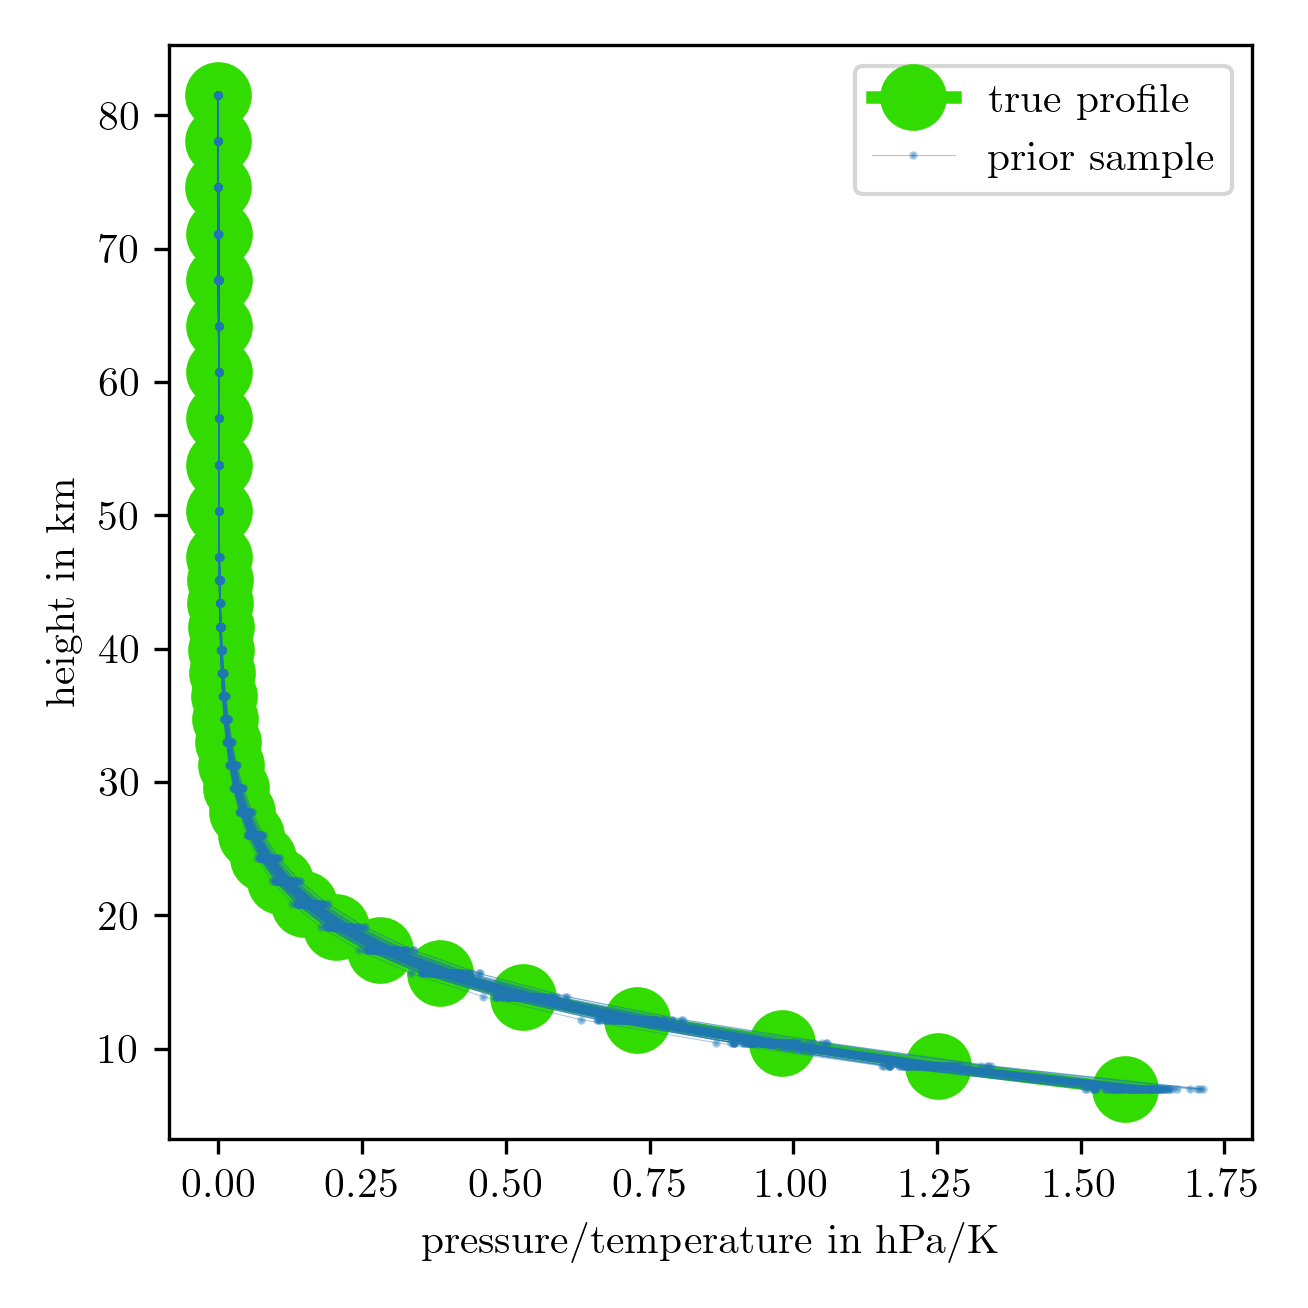
\includegraphics{PriorTempOverPostMeanSigm.png}
	\caption[Prior Samples of $\bm{p}/\bm{T}$ according to the respective hyper-prior distribution.]{We draw samples from the hyper-prior distribution of $h_0, b, p_0, h_1, h_2,h_3,h_4,h_5,h_6, a_0, a_1, a_2,a_3,a_4$ and $T_0$ as defined in table \ref{tab:priors} and then calculate $\bm{p}/\bm{T}$ according to the functions in Eq. \ref{eq:pressFunc} and \ref{eq:tempFunc}.}
	\label{fig:PriorPressOverTemp}
\end{figure}

\begin{figure}[ht!]
	\centering
	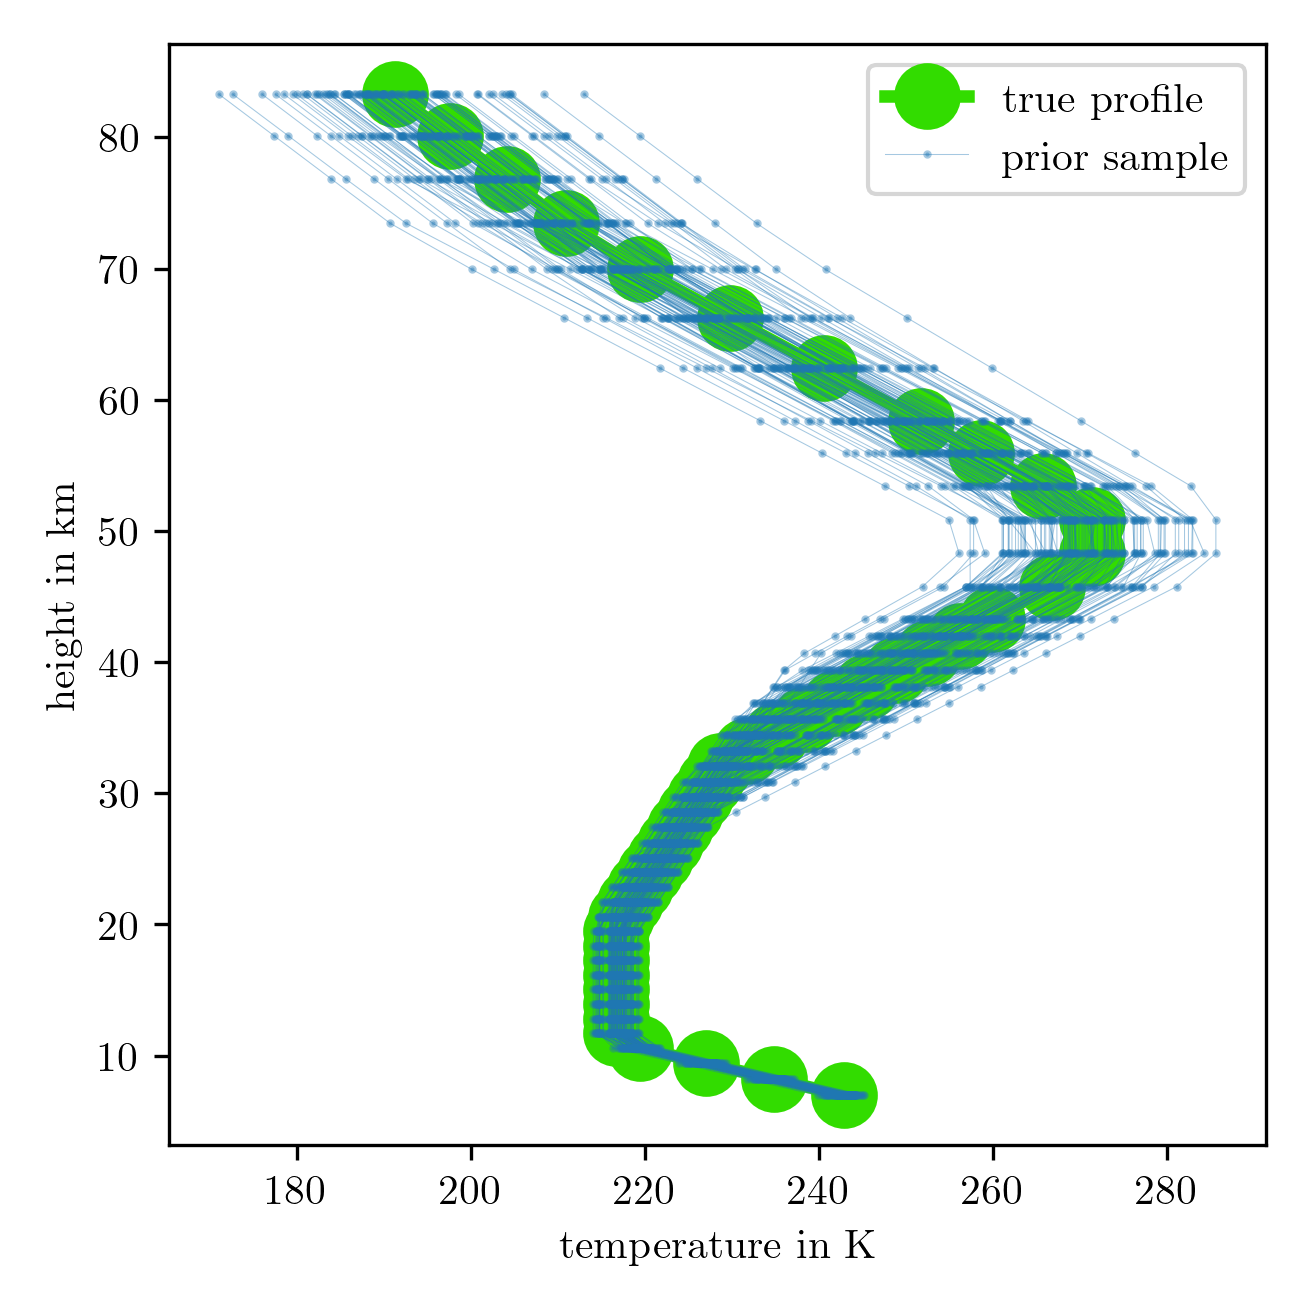
\includegraphics{PriorTempPostMeanSigm.png}
	\caption[Prior Samples of $\bm{T}$ according to the respective hyper-prior distribution.]{We draw samples from the hyper-prior distribution of $h_1, h_2,h_3,h_4,h_5,h_6, a_0, a_1, a_2,a_3,a_4$ and $T_0$ as defined in table \ref{tab:priors} and then calculate $\bm{T}$ according to the function in Eq. \ref{eq:tempFunc}.}
	\label{fig:PriorTemp}
\end{figure}

\begin{figure}[ht!]
	\centering
	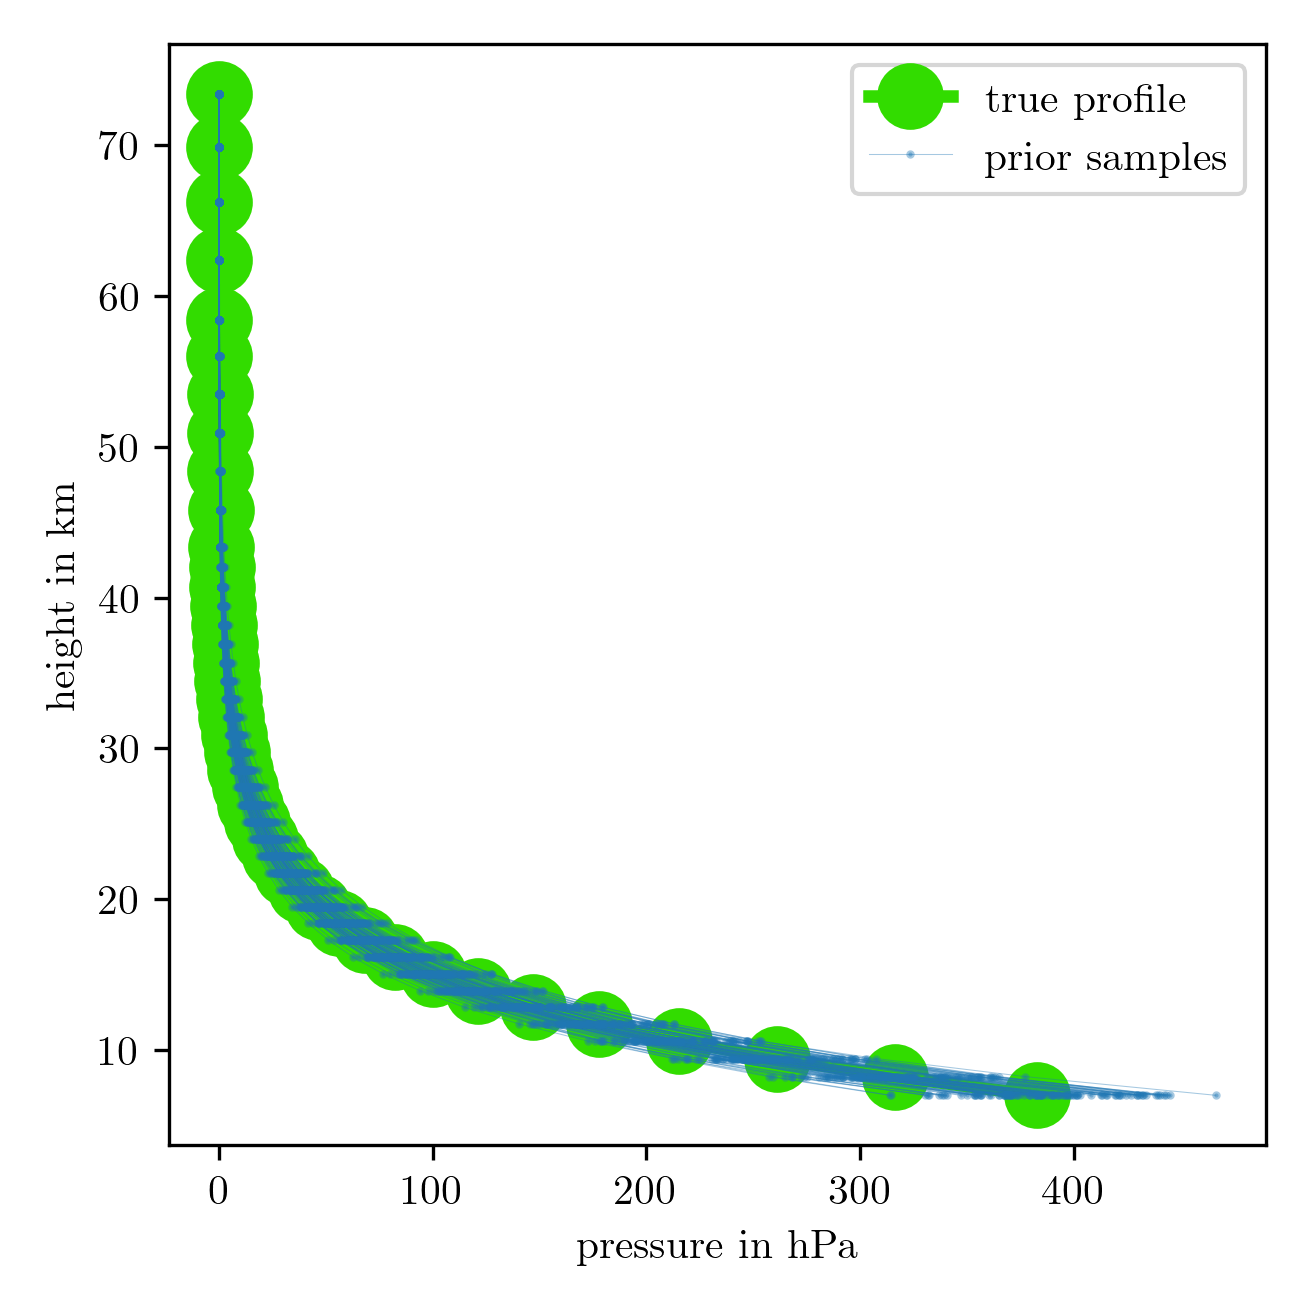
\includegraphics{PriorPressPostMeanSigm.png}
	\caption[Prior Samples of $\bm{p}$ according to the respective hyper-prior distribution.]{We draw samples from the hyper-prior distribution of $h_0, b$ and $p_0$ as defined in table \ref{tab:priors} and then calculate $\bm{p}$ according to the function in Eq. \ref{eq:pressFunc}.}
	\label{fig:PriorPress}
\end{figure}

\clearpage


\section{Posterior distributions with Linear model for Ozone -- MTC}
\label{sec:firstMTC}
In this section we calculate the posterior marginal and then conditional (MTC) posterior distribution for ozone conditioned on the ground truth temperature and pressure profiles using the linear forward model $\bm{A}_L$.
This is faster then the other way round (finding temperature over pressure conditioning on ozone) and temperature and pressure are well defined within the atmosphere so it is easier to just condition on a temperature and pressure profile out of a text book.
We employ a so-called Metropolis within Gibbs (MWG) algorithm on the marginal posterior as summarised in the algorithmic Box \ref{alg:margPost} or use a Tensor-Train (TT) approximation to calculate marginal posterior values.
Then we can either sample from the conditional posterior using the randomise then optimise (RTO) method or calculate conditional mean and variance using quadrature.

\begin{figure}[htb!]
	\centering
	\begin{tikzpicture}
		\node[roundnode2] at (-4,6.5) (Q)     {$\bm{Q}$};
		\node[roundnode2] at (-2.5,5) (x)     {$\bm{x}$};
		\node[align=center] at (-1,4) (A)    {$\bm{A}_L$};
		\node[roundnode2] at (-1,2.5) (u)    {$\bm{\Omega}$};
		\node[rectnode] at (-1,1) (y)    {$\bm{y}$};
		\node[roundnode2] at (-2.5,2.5) (e)    {$\bm{\eta}$};
		\node[roundnode2] at (-6.25,6.5) (S)    {$\bm{\Sigma}$};
		\node[roundnode2] at (-7.75,8) (s)    {$\gamma$};
		\node[roundnode2] at (-5.5,8) (d)    {$\delta$};
		
		%Lines
		\draw[->, very thick] (S.south east) -- (e.north west);
		\draw[->, mydotted, very thick] (s.south east) -- (S.north west);
		\draw[->, mydotted, very thick] (e.south east) -- (y.west);
		\draw[->, very thick] (u.south) -- (y.north);
		\draw[->, mydotted, very thick] (A.south) -- (u.north);
		\draw[->, mydotted,  very thick] (x.south east) -- (A.west);
		
		\draw[->, mydotted, very thick] (d.south east) -- (Q.north west); 
		
		\draw[->, very thick] (Q.south east) -- (x.north west); 
		%\node[align=center] at (0,4) (f3) {$= \bm{A}$};
		%\node[align=center] at (0.25,3.95) (f3) {$\approx \bm{M A}_L$};
		\node[align =center] at (-1,7) (T1) {marginal posterior \\ over hyper-parameters \\ $\pi(\gamma, \delta | \bm{y})$};
		\node[align =center] at (0,5) (T1) {conditional posterior \\ $\pi( \bm{x} |\gamma, \delta, \bm{y})$ };
		
		
		\node[fit=(S)(s)(Q)(d),draw,dotted,black, rounded corners] {};
	\end{tikzpicture} 
	\caption[Directed acyclic graph for ozone retrieval and MTC scheme.]{Directed acyclic graph for ozone retrieval and MTC scheme as described in Fig. \ref{fig:DAGComplete}. The hyper-parameters $\delta$ and $\gamma$ determine the noise covariance $\bm{\Sigma}$ for the random noise vector $\bm{\eta} \sim \mathcal{N}(0, \gamma^{-1}\bm{I})$ and the prior precision matrix $\bm{Q} = \delta \bm{L}$ for the distribution over $\bm{x} \sim \mathcal{N}(0, \delta \bm{L})$, where $\bm{L}$ is the graph Laplacian, see Eq. \ref{eq:GLapl}. In the MTC scheme we evaluate the marginal posterior over the hyper-parameters $\pi(\gamma, \delta | \bm{y})$ as in Eq. \ref{eq:} first and then conditional posterior $\pi(\bm{x}|\gamma,\delta,\bm{y})$ as in Eq. \ref{eq:}. The parameter$\bm{x}$ determine the space of all measurable noise free data $\bm{\Omega}$ through the forward model $\bm{A}(\bm{x},\bm{p},\bm{T})$ from which we randomly observe a data set plus some random noise.
		Note that once we found an affine map we update the forward model to $\bm{M}\bm{A}_L$.}
	\label{fig:DAGO3}
\end{figure}
The DAG in Fig. \ref{fig:DAGO3} visualises that process and we can show explicitly that we group the hyper-parameters $\delta, \gamma$ together to determine the marginal posterior $\pi(\gamma, \delta | \bm{y})$.
Here $\gamma$ , the noise parameter, determines the noise precision $\bm{\Sigma} = \gamma ^{-1} \bm{I}$ and $\delta$, the smoothness parameter, the precision matrix $\bm{Q} = \delta \bm{L}$ of the prior distribution for $\bm{x}$.
Then conditioned on the hyper-parameters the conditional posterior $\pi( \bm{x} |\gamma, \delta, \bm{y})$ gives the distribution of posterior ozone profiles.
Note that we use the linear model $A_L$ here as we do not have an approximation to the non-linear model yet and all prior distributions are defined in Table \ref{tab:priors}.
The full posterior $\pi(\bm{x},\gamma, \delta | \bm{y}) =  \pi(\bm{x}|\gamma, \delta ,\bm{y}) \pi(\gamma, \delta | \bm{y}) $ is given by multiplication of the marginal and conditional posterior densities. 

\subsection{Hyper-parameters samples from the marginal posterior distribution}
\label{subsec:firstMarg}
The marginal posterior distribution 
\begin{align}
	\pi(\lambda, \gamma | \bm{y})
	\propto  \lambda^{n/2} \gamma^{m/2}   \exp{ \Bigl\{ - \frac{1}{2} g ( \lambda) - \frac{\gamma}{2} f ( \lambda) \Bigr\} } \pi(\lambda, \gamma),
	\label{eq:MargPostAppl}
\end{align}
with $\lambda = \delta / \gamma$, and
\begin{subequations}
	\label{eq:fandg}
	\begin{align}
		&f ( \lambda) = \bm{y}^T \bm{y} - (\bm{A}_L^T \bm{y})^T (\bm{A}_L^T  \bm{A}_L + \lambda \bm{L})^{-1} (\bm{A}_L^T \bm{y})  \, ,  \\
		&\text{and } g(\lambda) = \log \det (\bm{A}_L^T  \bm{A}_L + \lambda \bm{L}) \, ,
	\end{align}
\end{subequations}
for the linear model $\bm{A}_L$, see Sec. \ref{subsec:MTC} for the derivation.
To calculate function values more efficiently we approximate the function $f(\lambda)$ and $g(\lambda)$ with 3rd order Taylor series around the mode $\lambda_0$ of $\pi(\lambda, \gamma | \bm{y})$, since the functions are well behaved over a large range of $\lambda$ see Fig. \ref{fig:fandg}.
The derivatives for the Taylor series are
\begin{align}
	f^{(r)}& (\lambda_0)= (-1)^{r+1} r! (\bm{A}_L^T \bm{y})^T (\bm{B}_0^{-1} \bm{L})^r \bm{B}_0^{-1} \bm{A}_L^T \bm{y} \label{eq:ftay}  \\
	\text{\textcolor{red}{include log(g) is linear}} &  g = g_0 \log{}
	%\text{and } &g^{(r)} ( \lambda_0) = (-1)^{r+1} \, \text{tr} \big( (\bm{B}_0^{-1}\bm{ L })^r \big)
	\label{eq:gtay}
\end{align} 
with $\bm{B}_0 = \bm{A}_L^T  \bm{A}_L + \lambda_0 \bm{L}$.
We find the mode at the minimum of  $-\log\{ \pi(\lambda, \gamma | \bm{y}) \}$  using \texttt{scipy.optimize.fmin} function and limit the number of function evaluation to 25 and use Cholesky back and forward substitution to calculate values of $g(\lambda)$ and $f(\lambda)$.
Additionally, we calculate $\bm{B}_0^{-1} \bm{L} $ and  $\bm{B}_0^{-1}  \bm{A}_L^T \bm{y}$ once more at $\lambda_0$ and plot the Taylor approximation within the sampling region in Fig. \ref{fig:fandg}.
\begin{figure}[ht!]
	\centering
	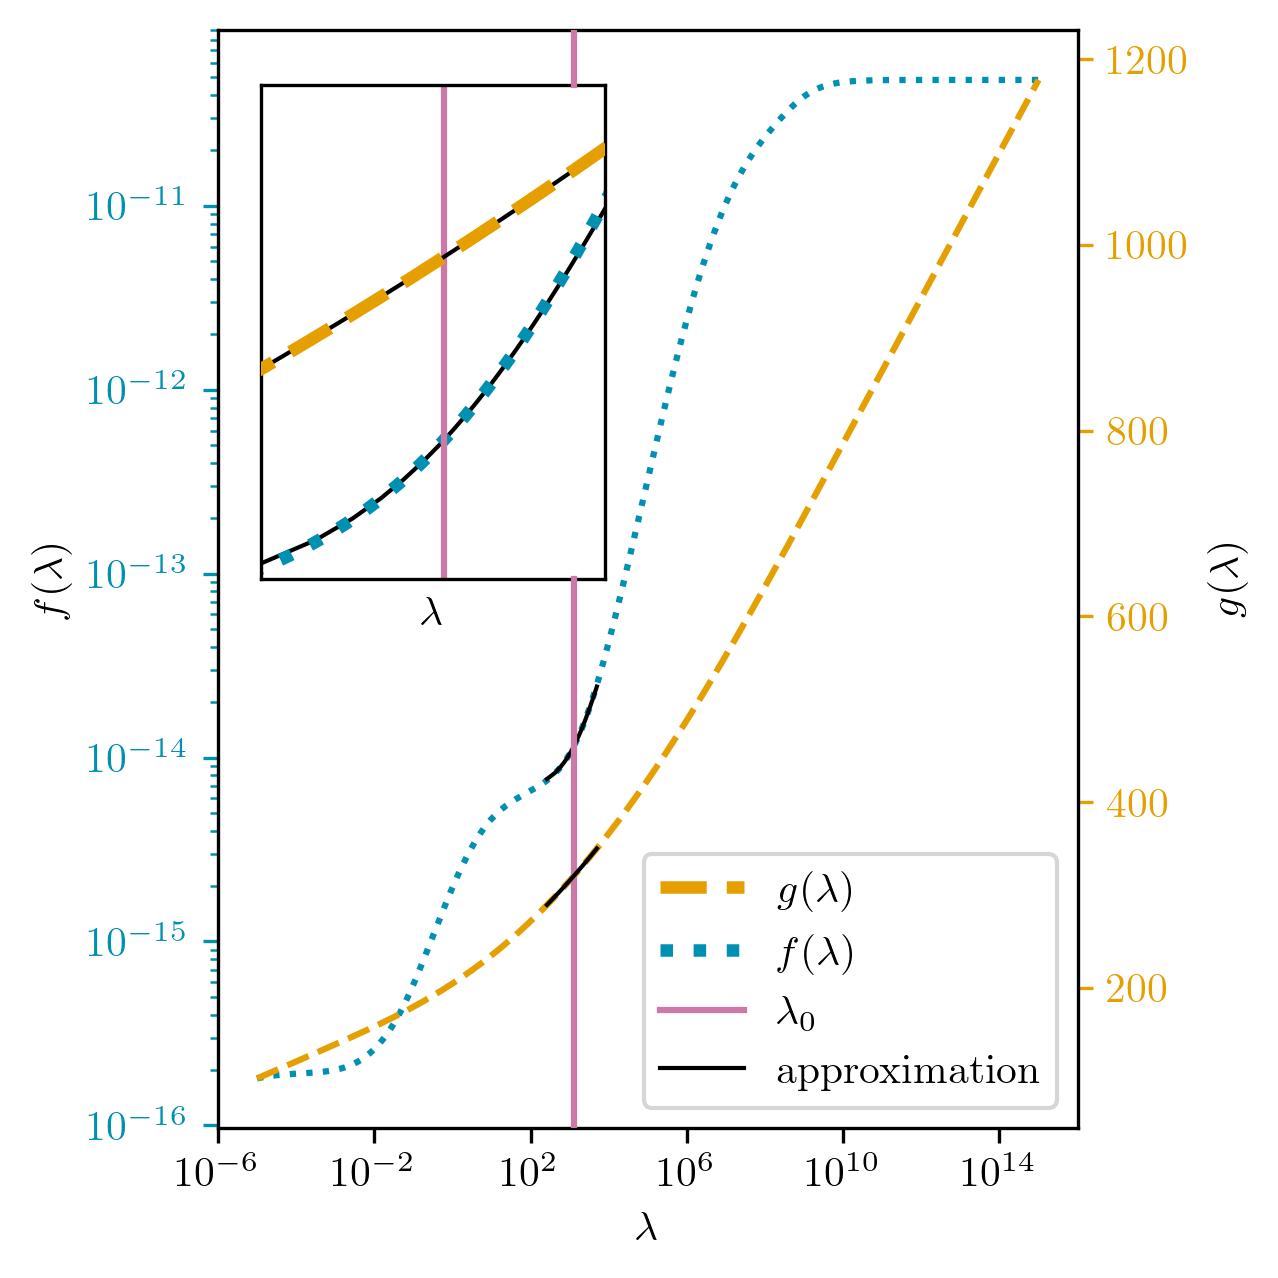
\includegraphics{f_and_g_phd.png}
	\caption[Plot of the functions $f(\lambda)$ and $g(\lambda)$ for marginal posterior.]{Plot of the functions $f(\lambda)$ and $g(\lambda)$ from the marginal posterior for a wide range of $\lambda = \delta / \gamma$. We plot the third order Taylor series in black around the mode of the marginal posterior (vertical line) for the sampling range of $\lambda$ within the MWG algorithm.}
	\label{fig:fandg}
\end{figure}



To characterise the marginal posterior function we employ a Metropolis within Gibbs (MWG) algorithm on $\pi(\lambda, \gamma | \bm{y})$.
In doing so, one may implement a Metropolis random walk on the full conditional
\begin{align}
	\label{eq:lamCondPrior}
	\pi(\lambda | \gamma, \bm{y}) &\propto \lambda^{n/2+\alpha_\delta -1} \exp{\Bigl\{ - \frac{1}{2} g ( \lambda) - \frac{\gamma}{2} f ( \lambda) - \beta_\delta \gamma \lambda \Bigr\}} 
\end{align} 
and do a Gibbs steps on
\begin{align}
	\gamma |  \lambda, \bm{y} &\sim \Gamma \bigg( \frac{m}{2} + \alpha_\delta + \alpha_\gamma, \frac{1}{2} f (\lambda ) + \beta_\gamma + \beta_\delta \lambda \bigg)\label{eq:GibbsStep}
\end{align} 
to generate marginal posterior samples $(\lambda, \gamma)^{(1)}, \dots, (\lambda, \gamma)^{(N)} \sim  \pi(\lambda, \gamma| \bm{y})$.
Note that, when changing variables from $\delta = \lambda \gamma$ to $\lambda$ the hyper-prior distribution changes to $\pi(\lambda) \propto \lambda^{\alpha_\delta-1} \gamma^{\alpha_\delta} \exp{(- \beta_\delta \lambda  \gamma)} $, due to $\text{d}\delta / \text{d} \lambda = \gamma$.

To run a Metropolis random walk on $\pi(\lambda | \gamma, \bm{y}) $ we choose a symmetric proposal distribution $q(\lambda^\prime|\lambda^{(k)}) \sim \mathcal{N}(\lambda^{(k)}, w_\lambda)$ conditioned on the previous sample $\lambda^{(k)}$, with $k = 1 , \dots, N$.
Here $N$ is the length of the output chain, but to insure that there are no biases due to the initialisation at the mode $( \lambda^{(0)} , \gamma^{(0)}  ) = ( \lambda_{0} , \gamma_{0}  )$  of the marginal posterior we discard the samples after a burn-in period $N_{\text{burn-in}}$.
So the effective output is  $N$ - $N_{\text{burn-in}}$.
To accept or reject a new sample $\lambda$ we draw a random uniform number in between 0 and 1 and compare with the acceptance ratio
\begin{align} 
	\log \left\{ \frac{\pi(\lambda | \gamma^{(t-1)}, \bm{y})  }{\pi(\lambda^{(t-1)}| \gamma^{(t-1)}, \bm{y})}  \right\} 
	= \log  \{\pi(\lambda | \gamma^{(t-1)}, \bm{y} ) \}  -\log  \{ \pi(\lambda^{(t-1)}| \gamma^{(t-1)}, \bm{y}) \} \\
	= \frac{n}{2} (\log\{\lambda\} - \log\{\lambda^{(t-1)}\} ) + \frac{1}{2} \Delta g + \frac{\gamma^{(t-1)}}{2} \Delta f  + \beta_\delta \gamma^{(t-1)} \Delta \lambda  \, ,
\end{align}
which we calculate in the log space.
Here $\Delta f = f(\lambda^\prime) - f(\lambda^{(k)}) = \sum f^{(r)} (\lambda_0)\Delta \lambda^\prime - \Delta \lambda^{(k)} $ and $\Delta g = g(\lambda^\prime) - g(\lambda^{(k)})= \sum g^{(r)} (\lambda_0)\Delta \lambda^\prime - \Delta \lambda^{(k)} $, where $\Delta \lambda^\prime = \lambda^\prime - \lambda_0 $ and $\Delta \lambda^{(k)} =  \lambda^{(k)} - \lambda_0$.


Lastly, a Gibbs step provides a new $\gamma^{(k+1)} \sim \gamma | \lambda^{(k+1)}, \bm{y}$, see Equation \eqref{eq:GibbsStep}.
See Algorithmic Box \ref{alg:margPost} for summarised version.
\begin{algorithm}[!ht]
	\caption{Metropolis within Gibbs for $\pi(\lambda, \gamma | \bm{y})$}
	\begin{algorithmic}[1]
		\STATE Initialise  \( \bm{\theta}^{(0)}  =( \lambda^{(0)} , \gamma^{(0)}  ) \) and set burn-in $N_{\text{burn-in}}$
		\FOR{ \( k = 1, \dots, N^{\prime} \)}
		\STATE Propose \( \lambda \sim \mathcal{N}(\lambda^{(t-1)}, 0.8 \lambda_0)  \)
		\STATE Compute
		\[ \alpha( \lambda  | \lambda^{(t-1)}) = \min \left\{ 1, \frac{\pi(\lambda | \gamma^{(t-1)}, \bm{y})  }{\pi(\lambda^{(t-1)}| \gamma^{(t-1)}, \bm{y})}  \right\} \]
		\STATE Draw $u \sim \mathcal{U}(0,1)$
		\IF{$\alpha \geq u$ }
		\STATE Accept and set \( \lambda^{(t)} = \lambda \)
		\ELSE  
		\STATE Reject and keep \(\lambda^{(t)} = \lambda^{(t-1)} \)
		\ENDIF
		\STATE Draw $\gamma^{(t)} | \lambda^{(t)} ,\bm{y} \sim \text{Gamma} \big( 0.5  \, m + 2, 0.5 \, f(\lambda^{(t)}) + 10^{-10}(1 + \lambda^{(t)}) \big) $
		\ENDFOR
		%\STATE Output: $ \bm{\theta}^{(N_{\text{burn-in}})}, \dots,  \bm{\theta}^{(k)} , \dots,   \bm{\theta}^{(N)} \sim \pi(\bm{\theta}| \bm{y}) $
		\STATE Output: $ (\lambda, \gamma)^{(N_{\text{burn-in}})}, \dots,  (\lambda, \gamma)^{(k)} , \dots,   (\lambda, \gamma)^{(N)} \sim \pi(\lambda, \gamma| \bm{y}) $
	\end{algorithmic}
	\label{alg:margPost}
\end{algorithm}



We run the MwG for $N = 20000$ plus $N_{\text{burn-in}} = 100$ steps and set the standard deviation of the normal proposal distribution to $\sigma_{\lambda} = 0.8 \lambda_0$ so that the acceptance rate is $\approx 0.5$ as suggested in \cite{}.
The samples are plotted in Fig. \ref{fig:ScatterPlotTT} as a 2D scatter plot, as well as the trace of the MwG to show ergodicity.


Alternatively we can approximate the square root of marginal posterior with a Tensor-Train (TT) on a grid as defined in table \ref{tab:priors} with $40$ grid points in each dimension.
Here we use the \texttt{rect\_cross.cross} as a black box algorithm from the \texttt{ttpy} python package, based on the rect cross algorithm in \cite{}.
We set the number of ranks to a constant value equal to four and optimse over those rankes with one sweep.
For numerical reasons,to avoid underflow, we have to add a constant $c = 460$, such as $\pi(\lambda | \gamma ,\bm{y}) = \exp\{ \log{\pi(\lambda | \gamma, \bm{y})} + c\}$.
We calculate the marginals $\pi(\lambda| \bm{y})$ and $\pi(\gamma| \bm{y})$ as in section \ref{}, with a constant $\gamma = 1e-5 $, and plot the TT approximation as a colour code on top of the obtained samples in the scatter plot in Fig. \ref{fig:ScatterPlotTT}.


The TT alforith with has nkber of funciton evaluaation set with constant rank r 
$( (D-2) r \times n\times r + 2  \times n \times r)2 \times n_{sweep}$
400 for TT marg
we set assume an absolute approximation error of $1$ so that we set $\gamma^{\prime} = 1 / \uplambda(\mathcal{X}) $

On a MacBook Pro from 2019 with 2.4 Ghz quadcore intel core i5 processor it takes $\lessapprox  0.1$s to find the Tensors to approximate the marginal posterior.
In comparisons the to run the MwG takes $\approx 0.7s$ for $N = 20000$ effective samples.
\textcolor{red}{integrated autocorrelation time, roughly efficient independent samples}
\begin{figure}[ht!]
	\centering
	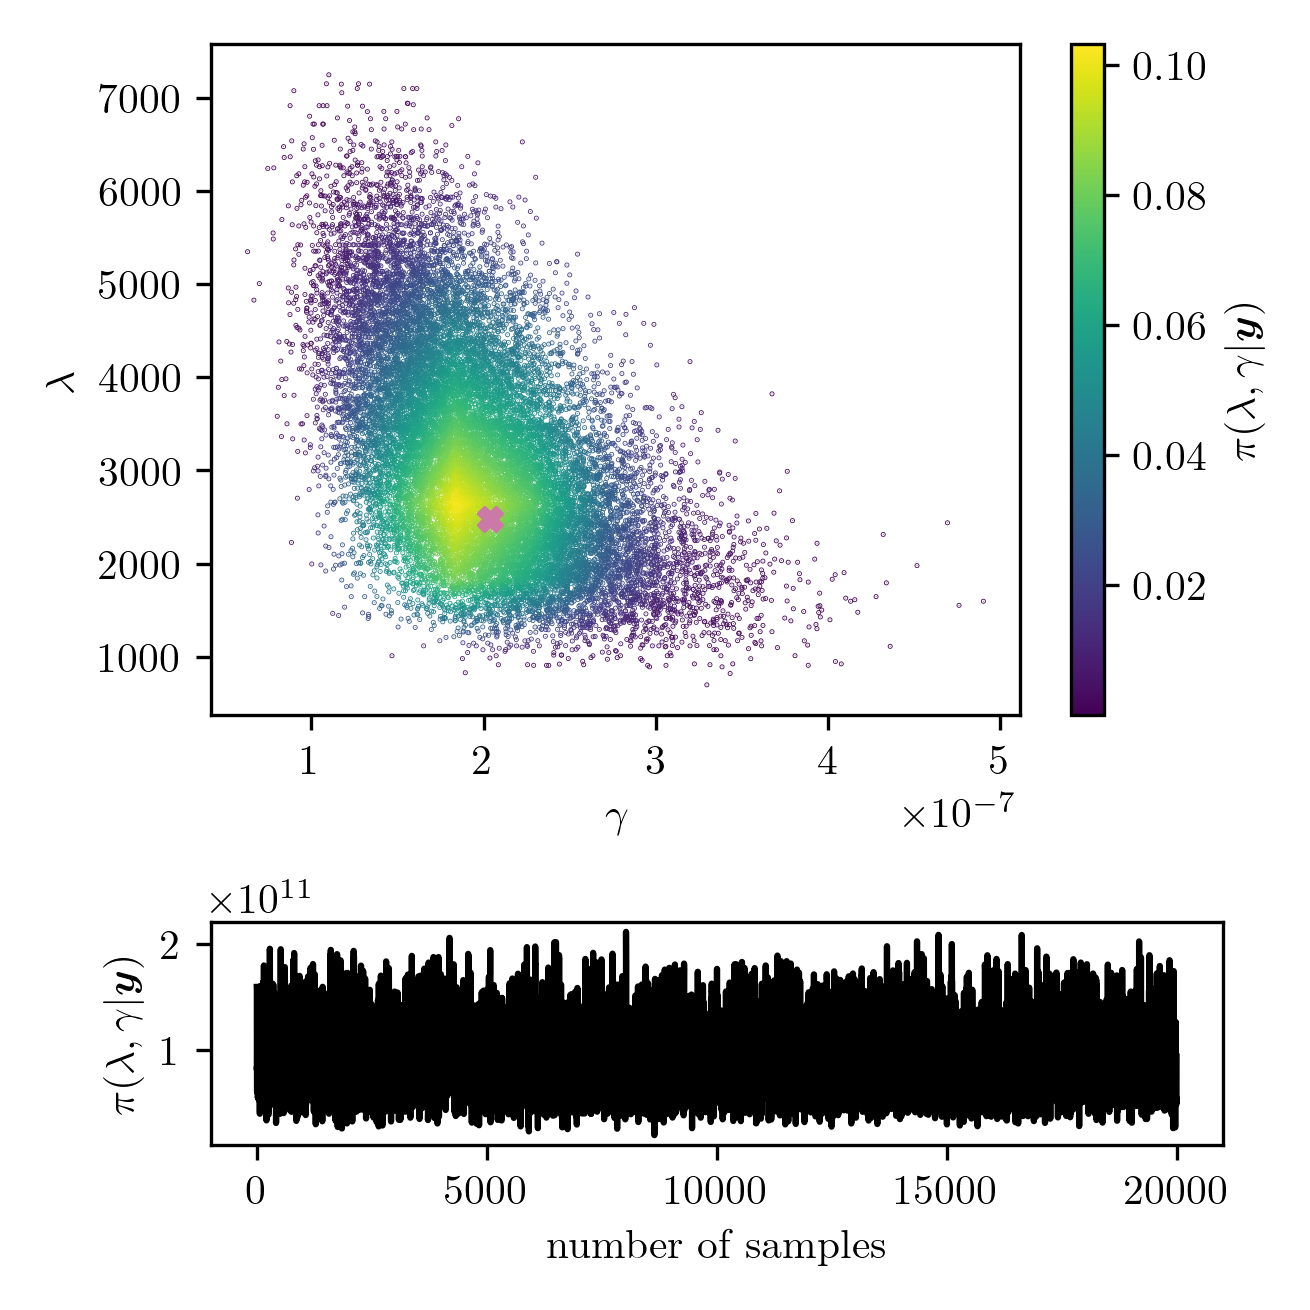
\includegraphics{ScatterplusHistoPlusTT.png}
	\caption[Scatter plot of samples from marginal posterior, including weighting from TT approximation; additional trace plot of the marginal posterior samples.]{We scatter plot the samples of $\lambda = \delta / \gamma $ and $\gamma$ from the marginal posterior $\pi(\lambda , \gamma  | \bm{y})$ and colour code the samples using the TT approximation of $\pi(\lambda , \gamma  | \bm{y})$. The mode of $(\lambda_0 , \gamma_0)$ of $\pi(\lambda , \gamma  | \bm{y})$ provided by \texttt{scipy.optimize.fmin} is marked with the cross. To show ergodicity we plot the trace of the samples of the Metropolis-within-Gibbs sampler below.}
	\label{fig:ScatterPlotTT}
\end{figure}

\textcolor{red}{Error Analysis?}
\subsubsection{Error due to approximation of f and g}
Error due to approximatino (taylor f and linear g)
Propagation error in $\ln{\pi(\lambda,\gamma|\bm{y})}$
propagation error in $\pi(\lambda,\gamma|\bm{y})$
3rd order taylor gives least error
error lays in the tails of distribution and we do not see a difference in tails
or ozone profiles

Can reduce error approximating at the mode currently we could approximate at the man e.g. the mean since it is a skewed distribution


\subsection{Ozone samples from the conditional posterior}
\label{subsec:firstCond}
As part of the MTC scheme we draw ozone samples after determining the marginal posterior distribution.
In this section we present two ways to draw ozone samples from the conditional posterior
\begin{align}
	\bm{x}| \delta, \gamma, \bm{y}  \sim \mathcal{N}\big( \underbrace{ (\bm{A}_L^T \bm{A}_L + \delta / \gamma \bm{L} )^{-1} \bm{A}_L^T \bm{y}}_{\bm{x}_{\lambda}}, ( \underbrace{ \gamma \bm{A}_L^T \bm{A}_L + \delta \bm{L} }_{\gamma \bm{B}_{\lambda}}  )^{-1} \big) \, \label{eq:CondPost}.
\end{align}
First we present the Randomize-than-Optimize (RTO) method \cite{bardsley2012mcmc,bardsley2015randomize, fox2016fast}, as previously described in Sec. \ref{subsec:RTO}.
Alternatively we can integrate over the marginal posterior and calculate the mean and variance of the multivariate normal conditional posterior distribution.
Note that we reject samples from the conditional posterior with negative ozone values since that is unphysical.

\subsubsection{Randomize then optimize -- RTO}
For the RTO method we start by drawing an independent hyper-parameter sample $ ( \delta, \gamma) \sim \pi(\delta, \gamma | \bm{y})$ from the samples of the MwG.
Then we generate two independent Gaussian random variables $\bm{v}_1 \sim \mathcal{N}(\bm{0},\gamma  \bm{A}^T_L \bm{A}_L)$ and $\bm{v}_2 \sim \mathcal{N}(\bm{0}, \delta \bm{L})$.
Here  can use Cholesky factorisation of $\bm{L}$ and the multiplication rule for normal distributions so that $\bm{v}_1 \sim \sqrt{\delta} \bm{L}_C \mathcal{N}(0,\bm{I})$ and $\bm{v}_2 \sim \sqrt{\gamma} \bm{A}_L^T \mathcal{N}(0,\bm{I})$.
Then we solve
\begin{align}
	\label{eq:FirstRTO}
	\left( \gamma \bm{A}_L^T  \bm{A}_L +\delta \bm{L} \right) \bm{x} = \gamma \bm{A}_L^T \bm{y} + \bm{v}_1 + \bm{v}_2 \, ,
\end{align}
using Cholesky back and forward substitution, for $\bm{x}$ and obtain one independent sample of $\pi(\bm{x}|\bm{y}, \bm{\theta})$.
See Fig. \ref{fig:O3Samp}, where we plot $m = $ samples of the conditional posterior.

The histogram in is binned as we intergate over it to 7 bins

\subsubsection{Weighted Mean}
Alternatively, we can calculated the mean
\begin{align}
	\mu_{\bm{x}|\bm{y}} = \int \bm{x}_{\lambda} \pi(\lambda| \bm{y}) \text{d}\lambda \approx \sum \bm{x}_{\lambda_i} \pi(\lambda_i| \bm{y}) \, , \label{eq:MeanInt}
\end{align} and covariance
 \begin{align}
 	\Sigma_{\bm{x}|\bm{y}} = \int \gamma^{-1}  \pi(\gamma | \bm{y} ) \, \text{d} \gamma \, \int  \bm{B}_{\lambda}^{-1} \, \pi(\lambda | \bm{y} )  \, \text{d} \lambda  \approx \sum {\gamma_i}^{-1}\pi(\gamma_i| \bm{y}) \sum \bm{B}_{\lambda_i}^{-1}\pi(\lambda_i| \bm{y})\, \label{eq:CovInt}
 \end{align}
of the conditional posterior $\pi(\bm{x}| \delta, \gamma, \bm{y})$, see Eq. \ref{eq:CondPost}, by quadrature \cite[Sec. 2.1]{Dick_Kuo_Sloan_2013}
We get function values for the marginal posterior either by binning the samples in Fig. \ref{fig:ScatterPlotTT} into a normalised histogram and use the height of the bars as quadrature weights, e.g. $\pi(\lambda_i| \bm{y})$, where $\lambda_i$ is at the centre of each bin, or from the TT approximation of $\sqrt{ \pi(\gamma, \delta | \bm{y}) }$, see also Fig. \ref{fig:MargPostHistTT}.
The integral can be interpreted as the weighted average, with $\sum \pi(\lambda_i| \bm{y}) = 1$ for normalised marginal functions.

If using the samples from the MWG algorithm, we start by binning the samples into $3$ bins and stop increasing the number of bins by one if the relative error between the previous and the current conditional posterior mean is less than $0.1\%$.
This happens at a bin number of $5$ and gives gives a total number of $3+4+5 = 12$ solves of $x_{\lambda}$ to find the conditional mean $	\mu_{\bm{x}|\bm{y}}$.
To calculate calculate the covariance matrix $(\gamma \bm{B}_{\lambda})^{-1} $, we use Cholesky forward and backward substitution to invert $\bm{B}_{\lambda}$, solve the integral in Eq. \ref{eq:CovInt} $5$ times.

Using the TT approximation we consider every second grid point of the total $40$ grid points of $\pi(\lambda| \bm{y})$ and $\pi(\gamma| \bm{y})$, which means we solve the integrals in Eq. \ref{eq:MeanInt} and \ref{eq:CovInt} 20 times.
We plot the mean and variance in Figure \ref{fig:O3Samp}.


\begin{figure}[ht!]
	\centering
	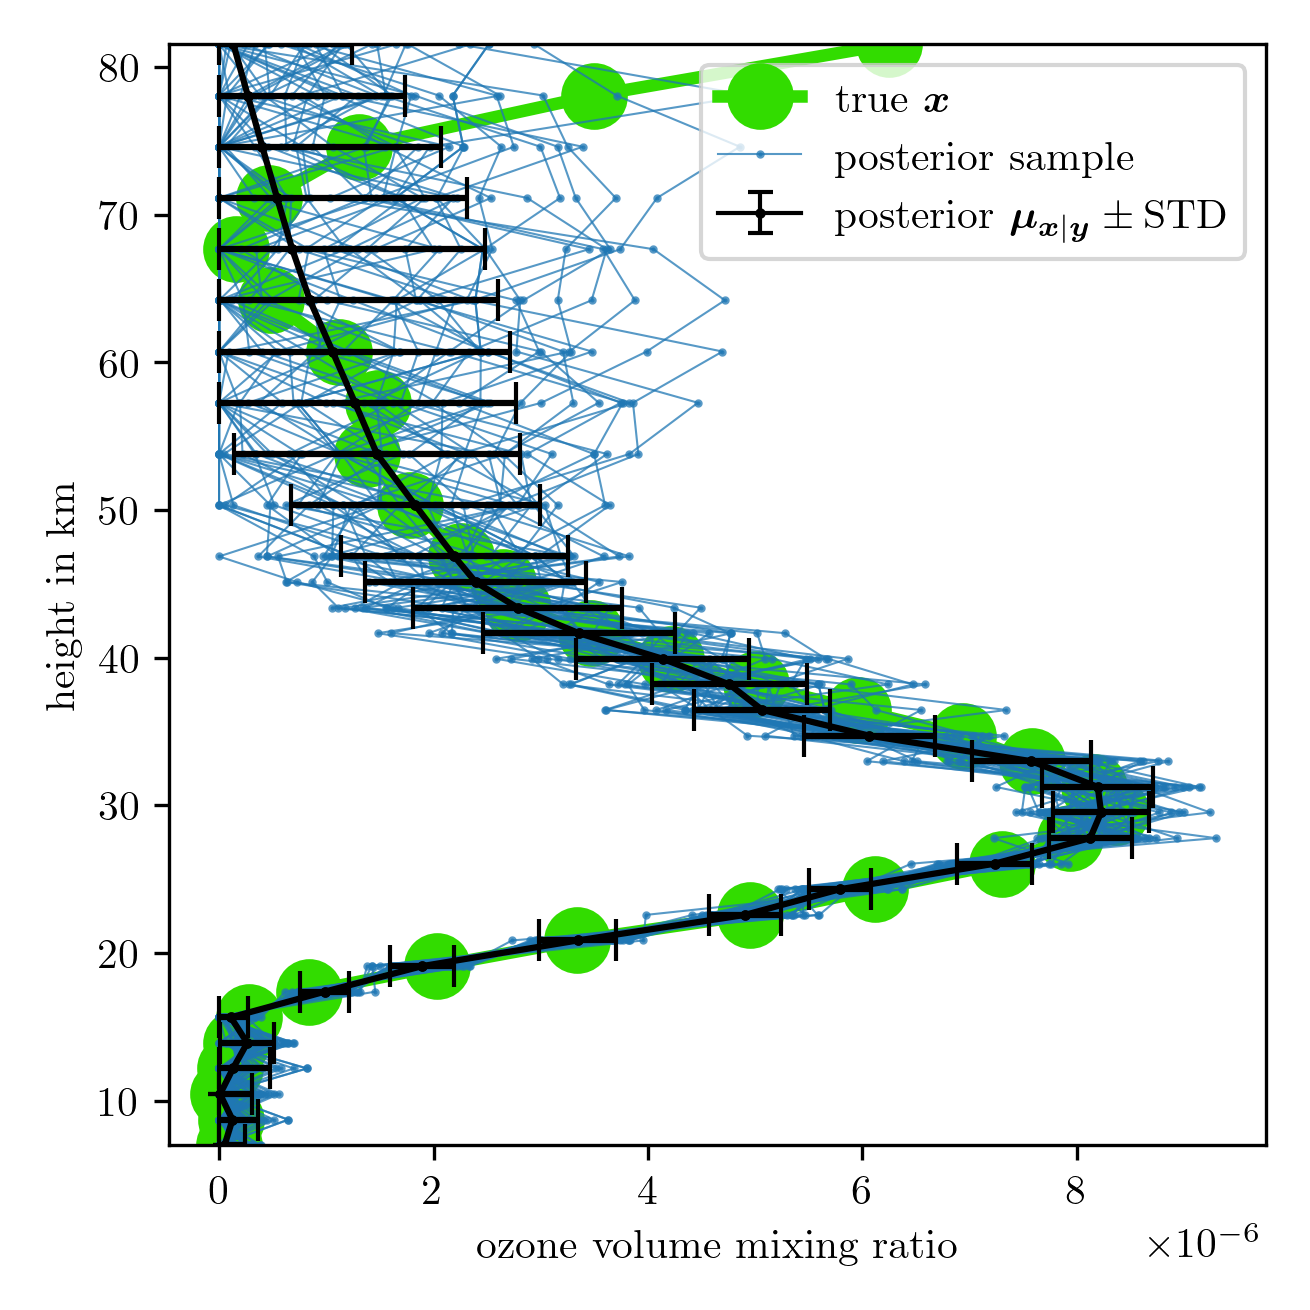
\includegraphics{FirstTestRes.png}
	\caption[Ozone samples of the conditional posterior.]{We draw samples from the conditional posterior distribution  $\pi(\bm{x}|\lambda,\gamma , \bm{y})$ after characterising the marginal posterior $\pi(\lambda,\gamma | \bm{y})$ through sampling or TT approximation using the linear forward map $\bm{A}_L$. Note that we reject samples with unphysical negative values and effectively treat the conditional posterior as a truncated multivariate normal distribution. We will use those samples to find the affine map $\bm{M}$, see section \ref{sec:affineMap}}
	\label{fig:O3Samp}
\end{figure}
\textcolor{red}{Error analysis and figure and argue TT gridsize}
\section{Approximate non-linear forward model with affine Map} 
\label{sec:affineMap}
Using an affine map to map in between the linear and non-linear forward map we can approximate the non-linear map and treat the inverse problem as a linear inverse problem.
In doing so we use the just calculated posterior distribution to generate ozone sample to generate noise free linear and non-linear data examples which we use to find the affine map.
\begin{figure}[htb!]
	\centering
	\begin{tikzpicture}
		\node[rectnode] at (0,0) (Oy)    {$\bm{y}$};
		\node[roundnode2] at (0,-2) (x)     {$\bm{x}$};
		\node[rectnode] at (-1.75,-4) (NLy)    {$\bm{A}_{NL}\bm{x}$};
		\node[rectnode] at (1.75,-4) (y)    {$\bm{A}_L\bm{x}$};
		\draw[->, very thick] (Oy.south) -- (x.north); 
		\draw[->, very thick] (x.south west) -- (NLy.north); 
		\draw[->, very thick] (x.south east) -- (y.north); 
		\draw[->, very thick] (NLy.east) -- (y.west); 
		\node[align=center] at (1,0) (l1) {Data};
		\node[align=center] at (3.5,-2) (f2) {Ozone Profiles from $\pi(\bm{x}|\gamma, \lambda ,\bm{y}) $};
		\node[align=center] at (1.75,-1) (l1) {$\pi(\lambda , \gamma  | \bm{y})$ with $\bm{A}_L$};
		
		\node[align=center] at (-4.75,-4) (f3) {non-linear forward model};
		\node[align=center] at (4.25,-4) (f4) {linear forward model};
		\node[align=center] at (0,-5) (f5) {$\bm{A}_{NL} \approx \bm{M A}_L= \bm{A}$ };
		
		\node[align=center] at (0,-4) (f5) {affine Map \\ $\bm{M}$};
		
	\end{tikzpicture}
\caption[Strategy to find affine map.]{The strategy to find the affine map consist of evaluating the marginal posterior for ozone using the linear forward model. Then we draw ozone samples from the conditional posterior and calculate noise free data based on the linear and non-linear forward model. Next we find a mapping in between those two space so that we can approximate the non-linear forward model using an affine map and the linear forward model.}
\end{figure}

With the samples $\{\bm{x}^{(1)} ,\dots, \bm{x}^{(m)}\}\sim \pi(\bm{x}|, \gamma, \lambda, \bm{y}) $ from the conditional posterior we generate two affine subspaces
\begin{align}
	\bm{V} = \begin{bmatrix}
		\vert&   &  \vert & & \vert \\
		\bm{A}_{NL} (\bm{x}^{(1)} ) &  \cdots& \bm{A}_{NL} (\bm{x}^{(j)} )&  \cdots & \bm{A}_{NL} (\bm{x}^{(m)})  \\
		\vert&   &  \vert & & \vert 
	\end{bmatrix} = 
	\begin{bmatrix}
		\rule[.5ex]{1em}{0.4pt} & v_1 &	\rule[.25ex]{1em}{0.4pt}\\
		&\vdots  & \\
		\rule[.5ex]{1em}{0.4pt} &v_j &	\rule[.25ex]{1em}{0.4pt}\\
		&\vdots  & \\
		\rule[.5ex]{1em}{0.4pt}& v_m&	\rule[.25ex]{1em}{0.4pt}
	\end{bmatrix} \, ,
\end{align} 
using the non-linear forward model, and 
\begin{align}
	\bm{W} = \begin{bmatrix}
		\vert&   &  \vert & & \vert \\
		\bm{A}_{L} \bm{x}^{(1)} &  \cdots& \bm{A}_{L} \bm{x}^{(j)} &  \cdots & \bm{A}_{L} \bm{x}^{(m)} \\
		\vert&   &  \vert & & \vert 
	\end{bmatrix}
\end{align}
based on the linear forward model, which are matrices in $\mathbb{R}^{m \times m}$.
To find the affine map \begin{align}
	\bm{M} = \begin{bmatrix}
		\text{---} & r_0 &   \text{---}  \\
		&  \vdots  & \\
		\text{---}& r_j &  \text{---} \\
		&  \vdots  & \\
		\text{---} & r_m &   \text{---}
	\end{bmatrix} \, \in \mathbb{R}^{m \times m} ,
\end{align} we use the \texttt{numpy.linalg.solve} python function to solve
\begin{align}
	v_j = r_j \bm{W}
\end{align}
where $r_j$ is the j-th row of $\bm{M}$.


Finally, we approximate the non-linear forward model
\begin{align}
	\bm{A}_{NL} \approx \bm{M A}_L = \bm{A} \, ,
\end{align}
with the affine map $\bm{M}$ and the linear forward model $\bm{A}_L$.
In Fig. \ref{fig:MapAsses} we asses the affine map using one of the samples $\bm{x} \sim \pi(\bm{x}|, \gamma, \lambda, \bm{y}) $ from the conditional posterior and calculate the relative error $|| \bm{M}\bm{A}_L \bm{x} - \bm{A}_{NL} \bm{x} || / || \bm{M}\bm{A}_L \bm{x} ||$ in percent between the mapped noise free data and the noise free data based on the non-linear forward.
As displayed in Fig. \ref{fig:MapAsses} we can approximate the non-linear forward model well within the relative difference between the noisy data and noise free non-linear data which is approximately $ 1.7 \%$ and from here on will use the approximated forward map.
\begin{figure}[ht!]
	\centering
	%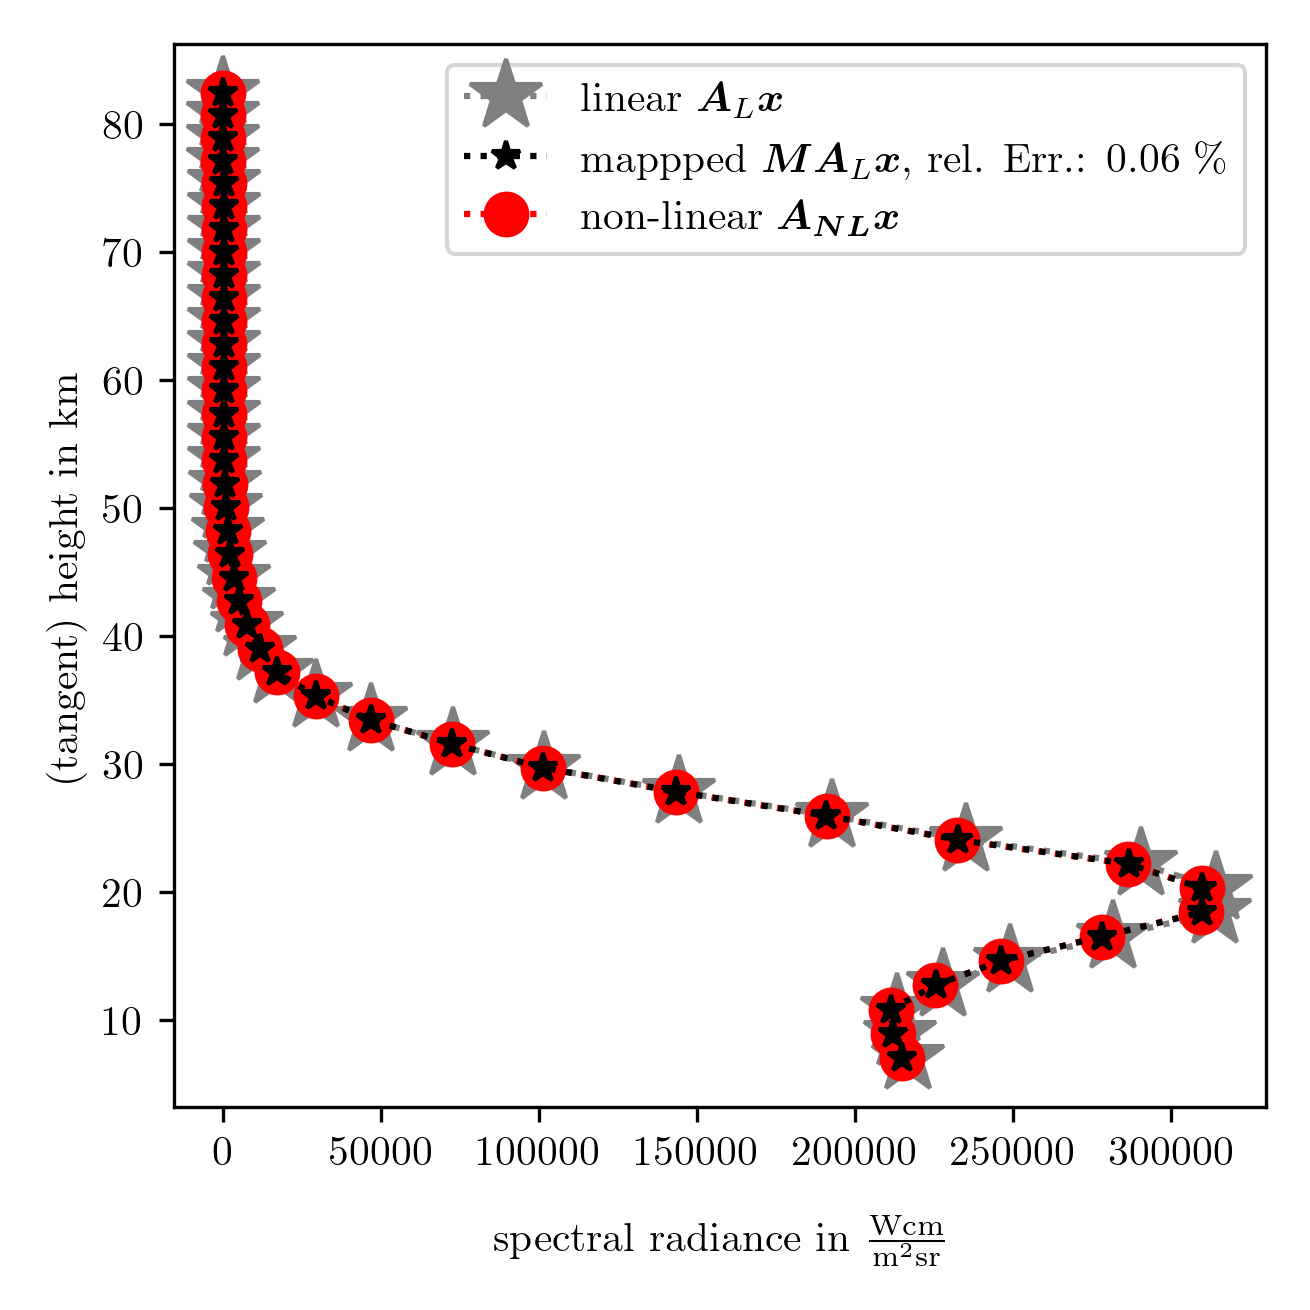
\includegraphics{SampMapAssesment.png}
	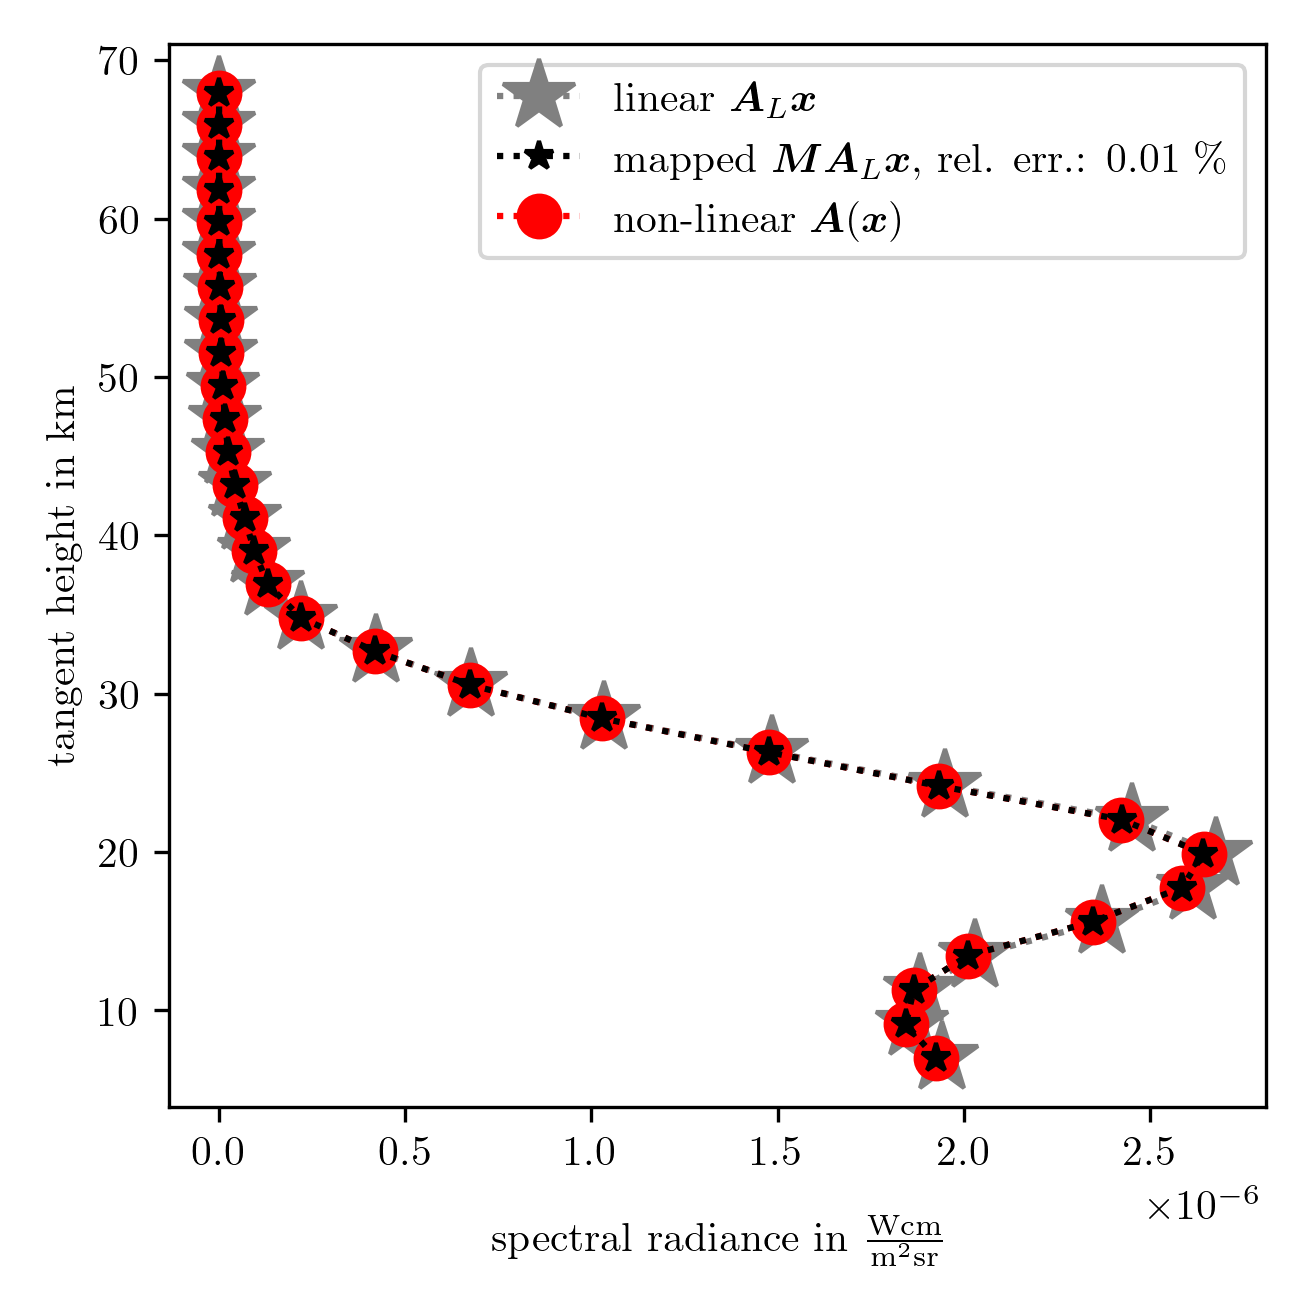
\includegraphics{SampMapAssesmentTT.png}
	\caption[Assessment of affine map.]{We asses how good we can map the linear forward model onto the non-linear forward model using the previous calculated affine map. The gray stars represent noise free linear data, where as the red circles present noise free non-linear data. Then we map the linear noise free data onto the non-linear noise free data and give the relative error in between the mapped noise free data and the non-linear data.}
	\label{fig:MapAsses}
\end{figure}



\section{Posterior distributions with approximated non-linear model for Ozone -- MTC}
From here on we use the approximation
\begin{align}
	 \bm{A} =  \bm{M A}_L \, 
\end{align}
of the non-linear forward map to be able to treat the problem as a linear inverse problem.
We use the exact same setup as in Sec. \ref{sec:firstMTC} but with the updated forward map $\bm{A}$.

\subsection{Hyper-parameters samples from the marginal posterior distribution}
With the updated forward map the marginal posterior distribution becomes
\begin{align}
	\pi(\lambda, \gamma | \bm{y})
	\propto  \lambda^{n/2} \gamma^{m/2}   \exp{ \Bigl\{ - \frac{1}{2} g ( \lambda) - \frac{\gamma}{2} f ( \lambda) \Bigr\} } \pi(\lambda, \gamma),
	\label{eq:UpdMargPostAppl}
\end{align}
with $\lambda = \delta / \gamma$, and
\begin{subequations}
	\label{eq:Updfandg}
	\begin{align}
		&f ( \lambda) = \bm{y}^T \bm{y} - (\bm{A}^T \bm{y})^T (\bm{A}^T  \bm{A} + \lambda \bm{L})^{-1} (\bm{A}^T \bm{y})  \, ,  \\
		&\text{and } g(\lambda) = \log \det (\bm{A}^T  \bm{A} + \lambda \bm{L}) \, .
	\end{align}
\end{subequations}
Again, we approximate the function $f(\lambda)$ and $g(\lambda)$ with 3rd order Taylor series around the mode $\lambda_0$ of $\pi(\lambda, \gamma | \bm{y})$, provided by \texttt{scipy.optimize.fmin}.
The Taylor derivatives are
\begin{align}
	f^{(r)}& (\lambda_0)= (-1)^{r+1} r! (\bm{A}^T \bm{y})^T (\bm{B}_0^{-1} \bm{L})^r \bm{B}_0^{-1} \bm{A}^T \bm{y} \label{eq:Updftay}  \\
	\text{and } &g^{(r)} ( \lambda_0) = (-1)^{r+1} \, \text{tr} \big( (\bm{B}_0^{-1}\bm{L})^r \big)
	\label{eq:Updgtay}
\end{align} 
with $\bm{B}_0 = \bm{A}^T  \bm{A} + \lambda_0 \bm{L}$.

We run the MWG algorithm and plot the samples in Fig. \ref{fig:MargPostHistTT} as well as the marginal approximations provided by the TT decomposition.
\begin{figure}[ht!]
	\centering
	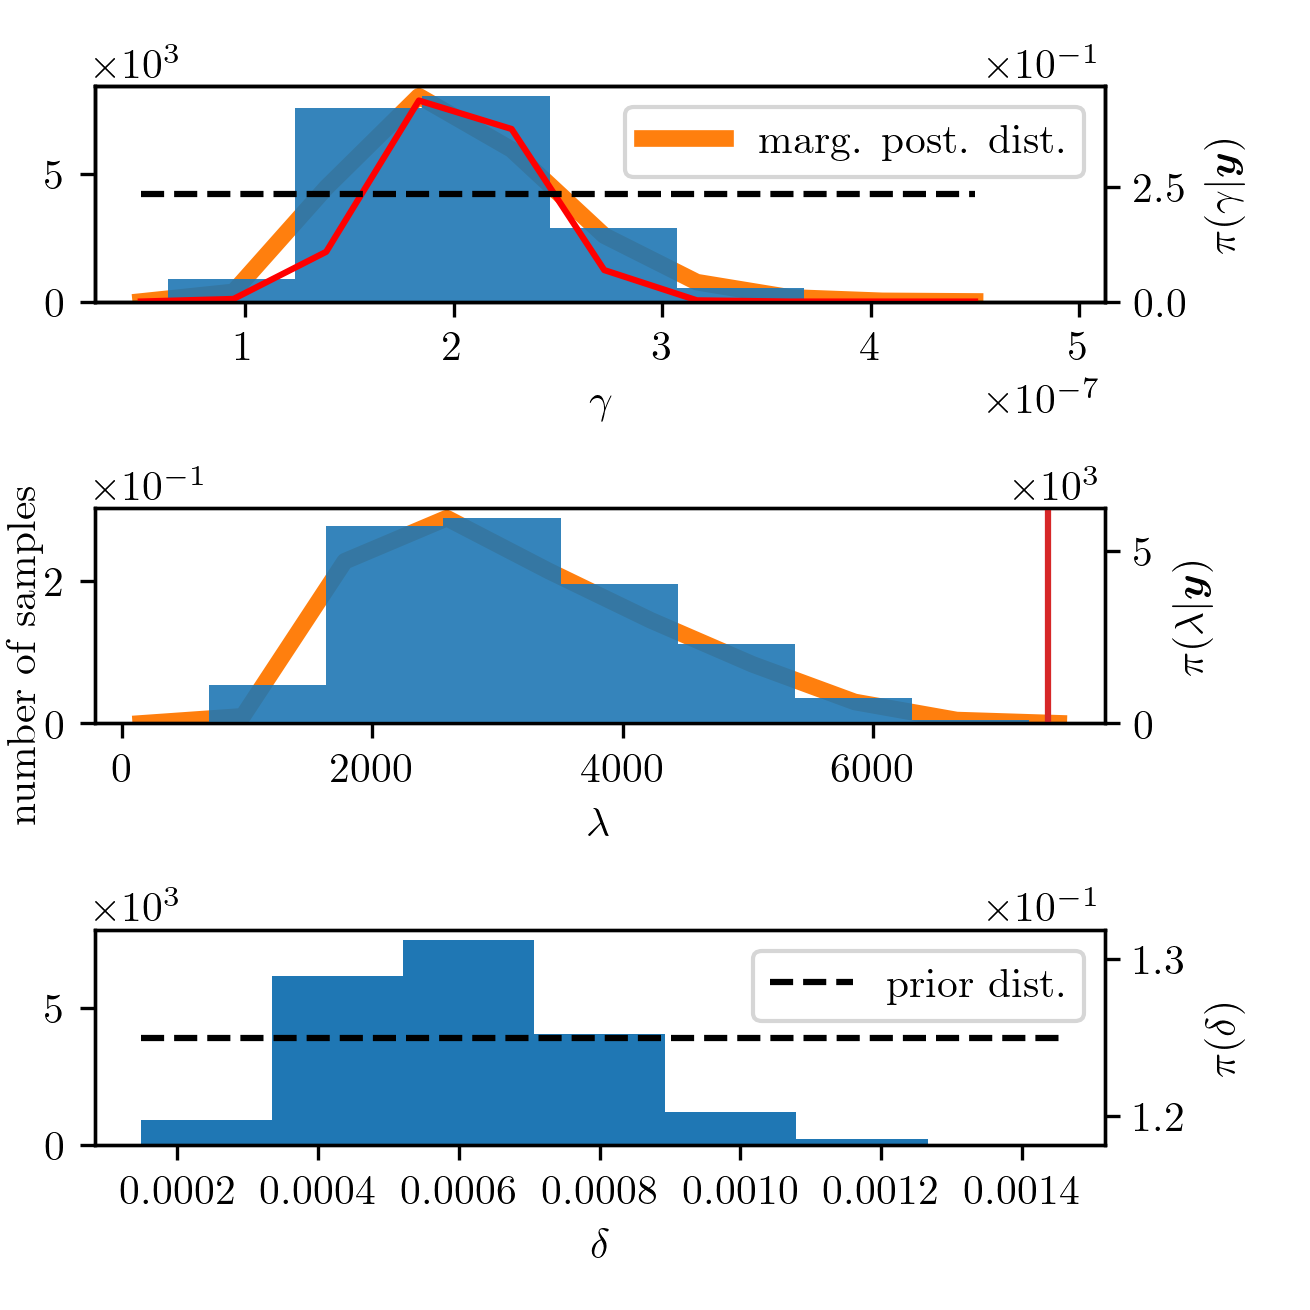
\includegraphics{secSIRTMargMargO3Res.png}
	\caption[Marginal posterior histograms and TT approximation as well as hyper-prior distribution.]{We plot the TT approximation of marginal posterior in orange and the samples as a histogram as well as the prior distribution with a dotted line. Note that we sample $\lambda$ and $\gamma$ using the Metropolis-within-Gibbs sampler and can calculate $\delta$ for every sample of the marginal posterior, we can not do this for the TT approximation. The regularised parameter corresponding to the regularised solution is marked thought the red vertical line at $\lambda_{\text{reg}} =$.}
	\label{fig:MargPostHistTT}
\end{figure}



\subsection{Ozone samples from the conditional posterior and regularised solution}
Next, we generate samples from the updated conditional posterior
\begin{align}
	\bm{x}| \delta, \gamma, \bm{y}  \sim \mathcal{N}\big( \underbrace{ (\bm{A}^T \bm{A} + \delta / \gamma \bm{L} )^{-1} \bm{A}^T \bm{y}}_{\bm{x}_{\lambda}}, ( \underbrace{ \gamma \bm{A}^T \bm{A} + \delta \bm{L} }_{\gamma \bm{B}_{\lambda}}  )^{-1} \big) \, \label{eq:UpdCondPost}
\end{align}
as described in Section \ref{subsec:firstCond}.

We plot the conditional mean and variance in Fig. \ref{fig:O3SolplsReg} and the regularised solution as well as one sample from the posterior.
\begin{figure}[ht!]
	\centering
	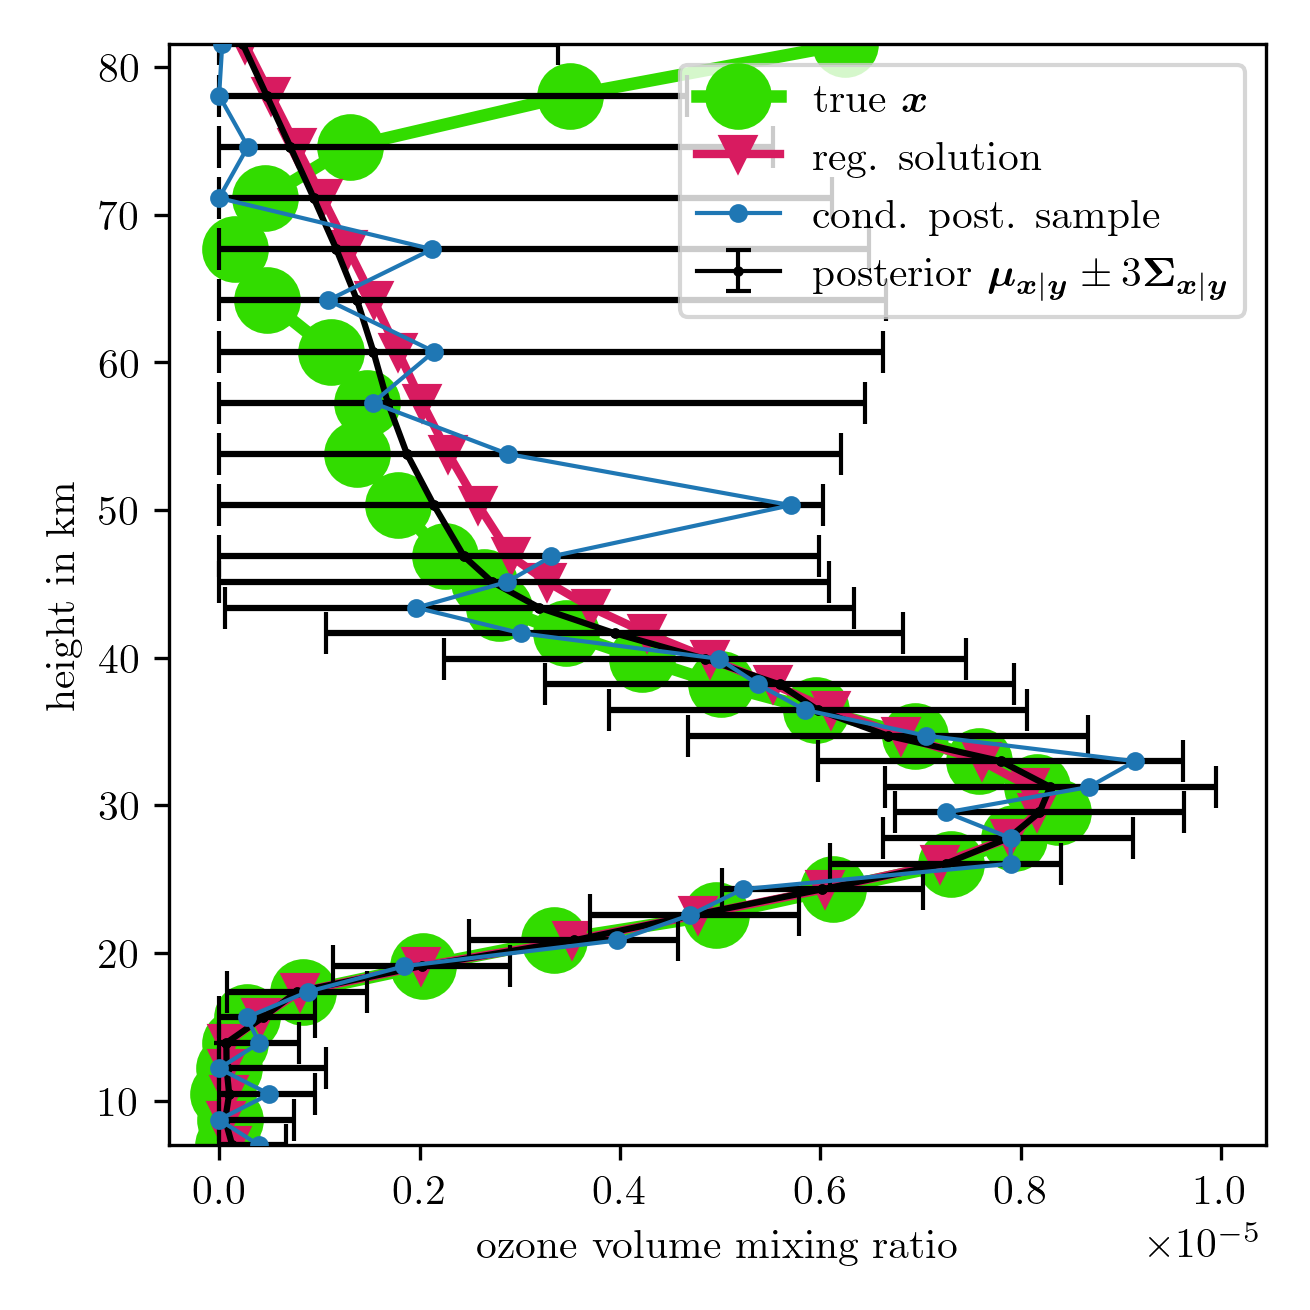
\includegraphics{SecRecResinclRegandSampl.png}
	%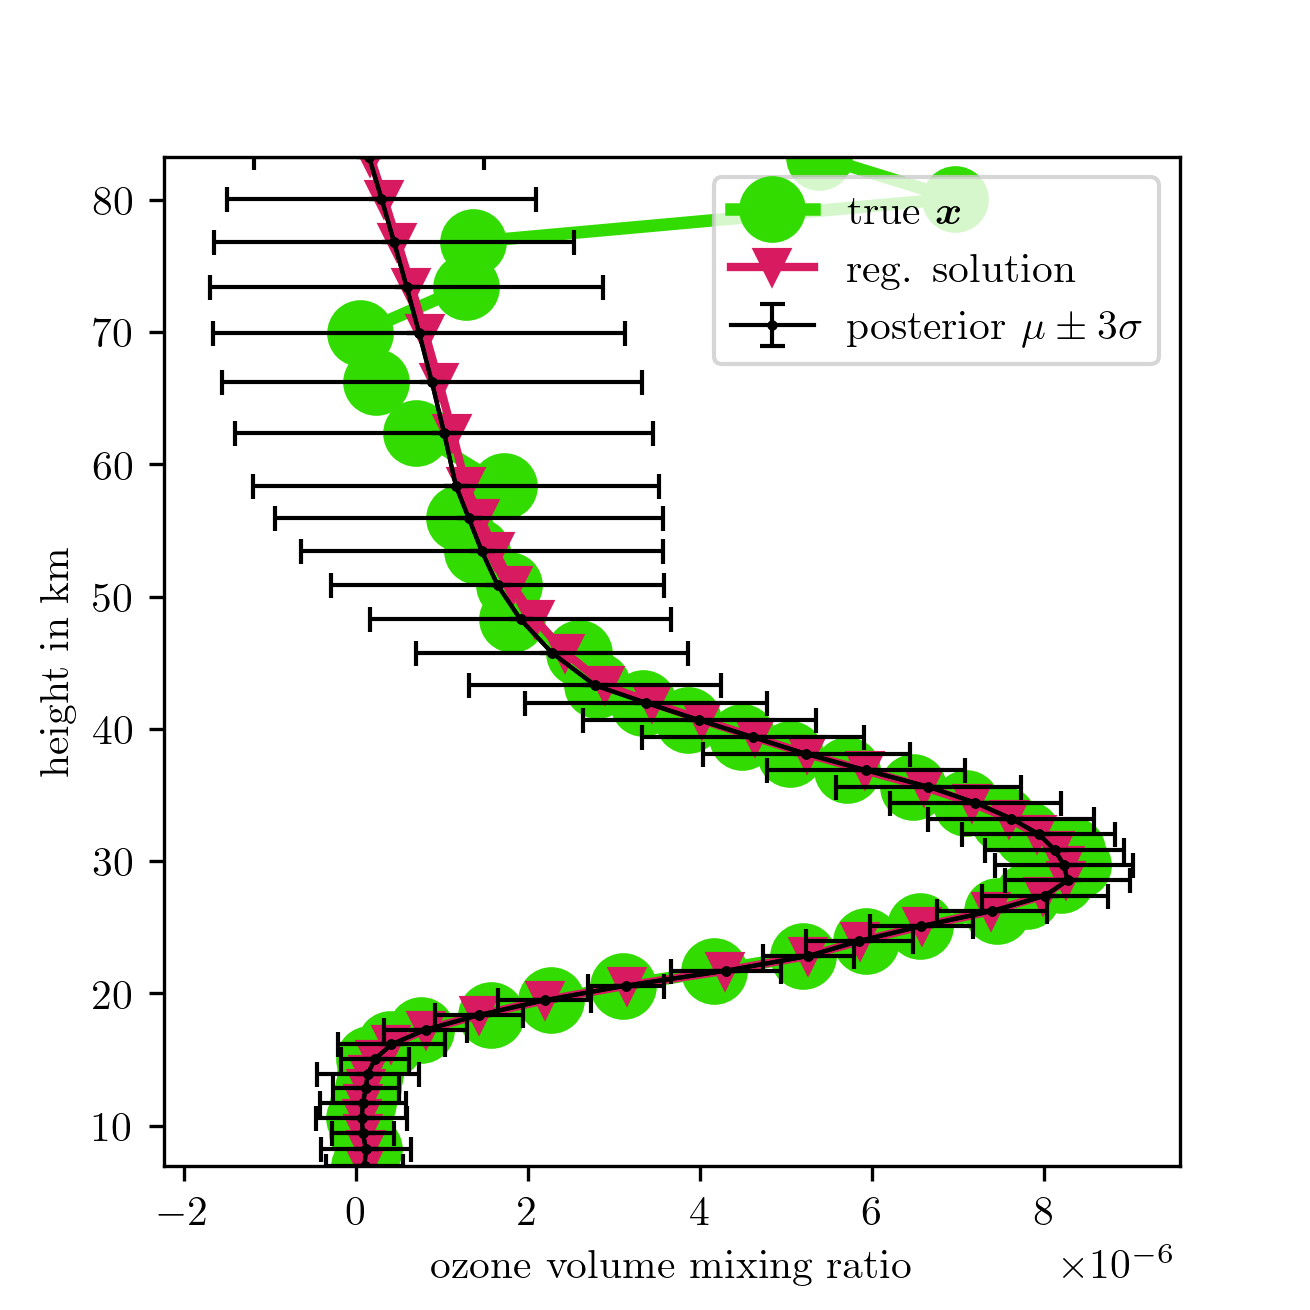
\includegraphics{SecRecResinclReg.png}
	\caption[Ozone posterior mean and variance and the regularised solution compared to the ground truth.]{We plot the conditional posterior mean and variance in black and the regularised solution on top of the ground truth ozone profile in green. We use the updated forward map $\bm{M}\bm{A}_L$}
	\label{fig:O3SolplsReg}
\end{figure}

\textcolor{red}{Data uninformative in higher altitude and say again reg sol. vs mean and one samples is good solution }


\subsection{Solution by regularisation}
\label{subsec:reg}
Additionally, we calculate a solution by Tikhonov regularisation as this is most similar to our chosen linear-Gaussian Bayesian framework.
The Tikhonov regularised solution is defined as~\cite{hansen2010discrete} 
\begin{align}
	\bm{x}_{\lambda} =\underset{ \bm{x}}{\arg \min}\,  \lVert \bm{A}\bm{x} - \bm{y} \rVert_2^2 + \lambda \bm{x}^T \bm{L} \bm{x} \, ,
	\label{eq:XLam}
\end{align}
with the regularisation parameter $\lambda = \delta / \gamma$.
This maximises the full conditional distribution for $\bm{x}$, so is not, as often erroneously stated, the maximum a posteriori (MAP) estimate which includes at the hyper-parameters.
The regularised solution is typically calculated by solving the normal equations, see Eq. \ref{eq:regSol},
\begin{align}
	\bm{x}_{\lambda} = (\bm{A}^T\bm{A} + \lambda \bm{L} )^{-1} \bm{A}^T \bm{y} \label{eq:xLam} \, .
\end{align}
In doing so we find the best regularisation parameter using the L-curve method~\cite{hansen1993use}.
Within this method we compute $\bm{x}_\lambda$, see Equation \eqref{eq:xLam}, for 200 different $\lambda$ values in between $1$ to $10^7$ and plot the solution semi norm $\sqrt{\bm{x}_\lambda^T\mathbf{L} \bm{x}_\lambda}$ against the data misfit norm $\lVert \bm{A}\bm{x}_\lambda - \bm{x} \rVert$, see Figure \ref{fig:LCurve}. 
The best regularised solution corresponding to the corner of the L-curve is located at the point of maximum curvature, see triangle in Fig. \ref{fig:LCurve}, which we find with the kneedle algorithm~\cite{satopaa2011kneedle} using the python function \texttt{kneed.KneeLocator}.
This takes roughly seconds on a MacBook Pro from 2019 with 2.4 Ghz quadcore intel core i5 processor.
\begin{figure}[ht!]
	\centering
	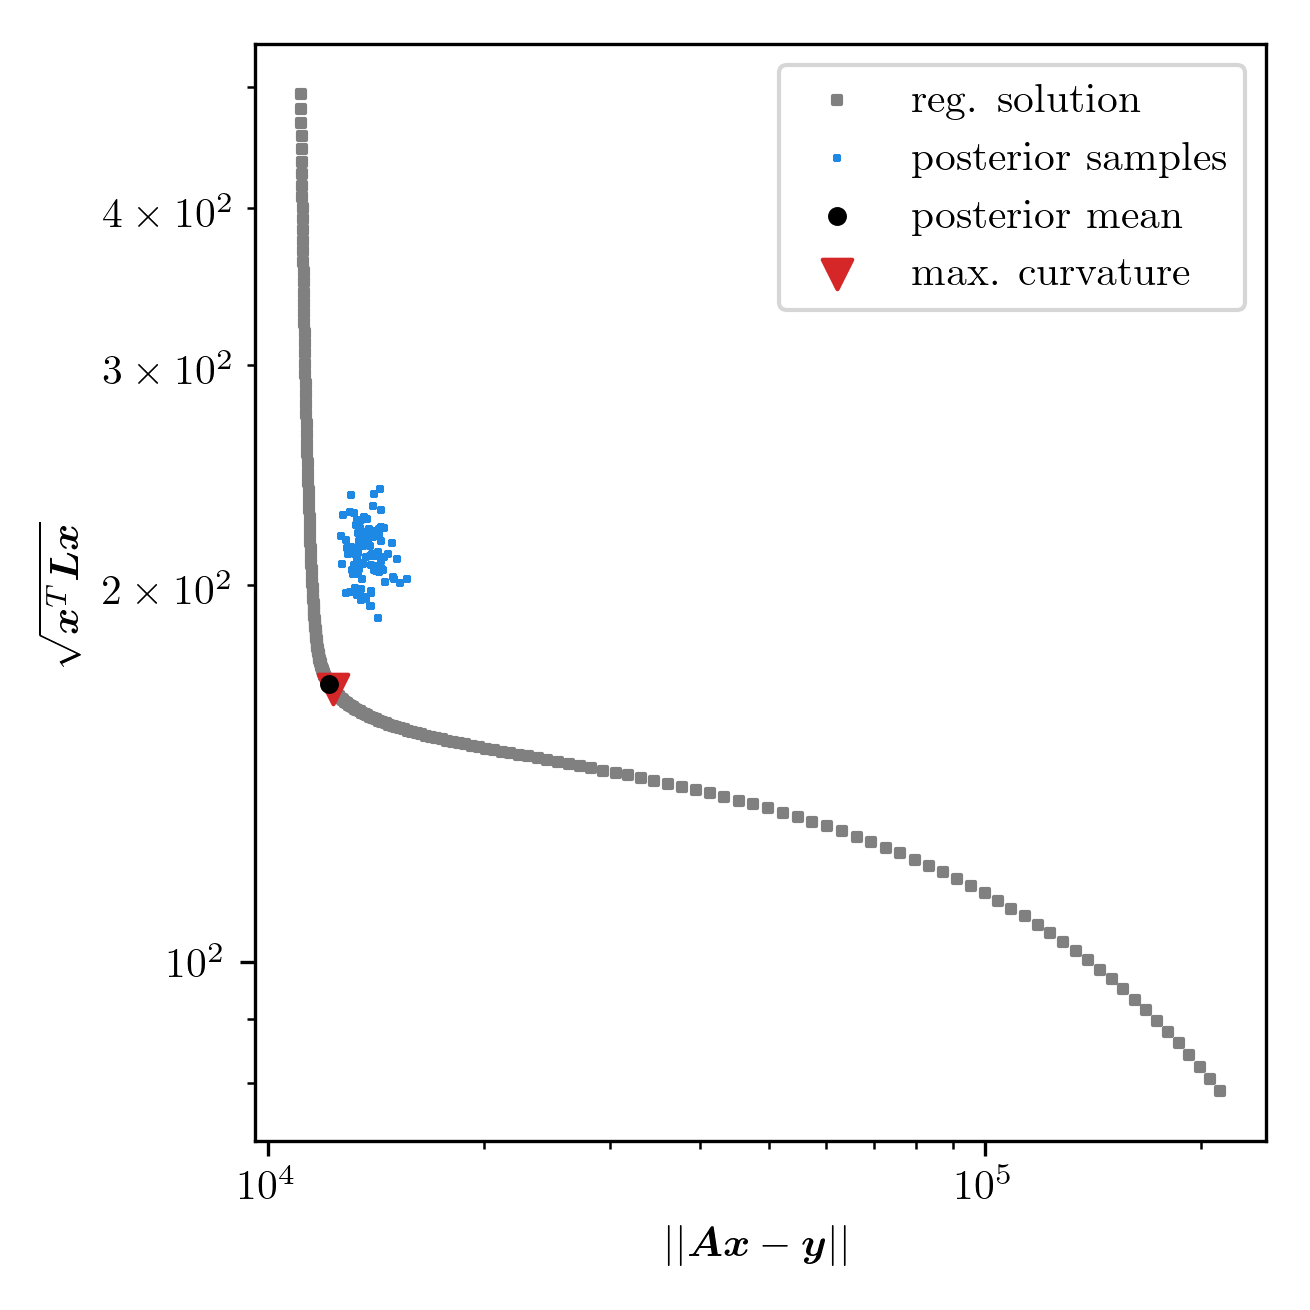
\includegraphics{LCurvePhD.png}
	\caption[Plot of the L-curve to find the regularised solution.]{We calculate regularised solution as in Eq. \ref{eq:} and plot the regularised semi norm $\sqrt{\bm{x}^T\bm{Lx}}$ against the data misfit norm $||\bm{Ax} -\bm{y} ||$ to find the regularised solution at the point of maximum curvature of the so-called L-Curve. Additionally we calculate the data misfit norm and the regularised norm for the ozone posterior and for samples of the conditional posterior distribution. \textcolor{red}{make box around Kneedle reagion}}
	\label{fig:LCurve}
\end{figure}

\textcolor{red}{Sol Reg vs Mean, vs samples, see L-Curve}





\section{Posterior pressure and temperature}
\label{sec:postPT}
\begin{figure}[thb!]
	\centering
	\begin{tikzpicture}
		
		\node[align=center] at (-1,4) (A)    {$\bm{M A}_L$};
		\node[roundnode2] at (-1,2.5) (u)    {$\bm{u}$};
		\node[rectnode] at (-1,1) (y)    {$\bm{y}$};
		
		\node[roundnode2] at (3,6.5) (t)     {$\bm{T}$};
		\node[roundnode2] at (-1,6.5) (p)     {$\bm{p}$};
		\node[roundnode2] at (1,5) (pt)     {$\bm{p}/\bm{T}$};
		\node[roundnode2] at (0,8) (b1)    {$b$};
		%\node[roundnode2] at (1,8) (b2)    {$b_2$};
		\node[roundnode2] at (-2,8) (h1)    {$h_0$};
		\node[roundnode2] at (-1,8) (p0)    {$p_0$};
		\node[roundnode2] at (2.25,8) (ht)    {$\bm{h}$};
		\node[roundnode2] at (3.25,8) (ct)    {$T_0$};
		\node[roundnode2] at (4.25,8) (at)    {$\bm{a}$};
		
		%Lines
		\draw[->, very thick] (u.south) -- (y.north);
		\draw[->, mydotted, very thick] (A.south) -- (u.north);
		
		\draw[->, mydotted, very thick] (p.south east) -- (pt.north west);
		\draw[->, mydotted, very thick] (t.south west) -- (pt.north east);
		\draw[->, mydotted, very thick] (pt.south west) -- (A.east);
		\draw[->, mydotted, very thick] (h1.south) -- (p.north west);
		\draw[->, mydotted, very thick] (p0.south) -- (p.north);
		\draw[->, mydotted, very thick] (b1.south) -- (p.north east); 
		%\draw[->, very thick] (b2.south) -- (p.east); 
		
		\draw[->, mydotted, very thick] (ht.south) -- (t.north west);
		\draw[->, mydotted, very thick] (ct.south) -- (t.north);
		\draw[->, mydotted, very thick] (at.south) -- (t.north east);
		
		\node[align =center] at (-5,8) (T1) {posterior \\ over hyper-parameters \\ $\pi(h_0, p_0, b, \bm{h}, T_0, \bm{a}| \bm{y})$};
		
		\node[fit=(h1)(at),draw,dotted,black, rounded corners] {};
	\end{tikzpicture} 
	\caption[Directed acyclic Graph for pressure and temperature.]{Conditioned on an ozone profile the posterior of the hyper-parameters describing pressure and temperature is given as in Eq. \ref{eq:}. Since pressure and temperature go into the forward model as $\bm{p}/\bm{T}$ they are highly correlated but the pressure is the dominant parameter, see Fig. 
		\ref{fig:PriorPressOverTemp} and \ref{fig:SeaLevelHist}. Note that here we use the updated forward model $\bm{M} \bm{A}_L$ and conditioned on a $\gamma$ sample from the previously evaluated marginal posterior see Fig. \ref{fig:MargPostHistTT}. }
	\label{fig:DAGPT}
\end{figure}

To find the posterior pressure and temperature we condition on a $\gamma$ sample, by fitting a normal distribution to either the samples or the TT approximation of $\pi(\gamma|\bm{y})$ plotted as a red line in Fig. \ref{fig:MargPostHistTT}, and the ozone sample plotted in \ref{fig:O3SolplsReg}, which is also used to find the affine map.
Consequently we use the updated forward map $\bm{A}= \bm{M}\bm{A}_L$ and the posterior is given by 
\begin{align}
	\begin{split}
	\pi(h_1,p_0,b_1,b_2,\bm{h_T},\bm{c_T},\bm{a_T} | \bm{y}, \gamma, \bm{x}) \propto  \exp\Bigl\{ & -\frac{\gamma}{2} \left\Vert \bm{y}- \bm{A} \frac{\bm{p}}{\bm{T}}  \right\Vert^2 \\ &+ \ln{\pi(h_1,p_0,b_1,b_2,\bm{h_T},\bm{c_T},\bm{a_T}) + c \Bigr\}  }
	\end{split} \, ,
\end{align}
where $c$ is a constant needed for the TT approximation to avoid underflow.

\begin{figure}[ht!]
	\centering
	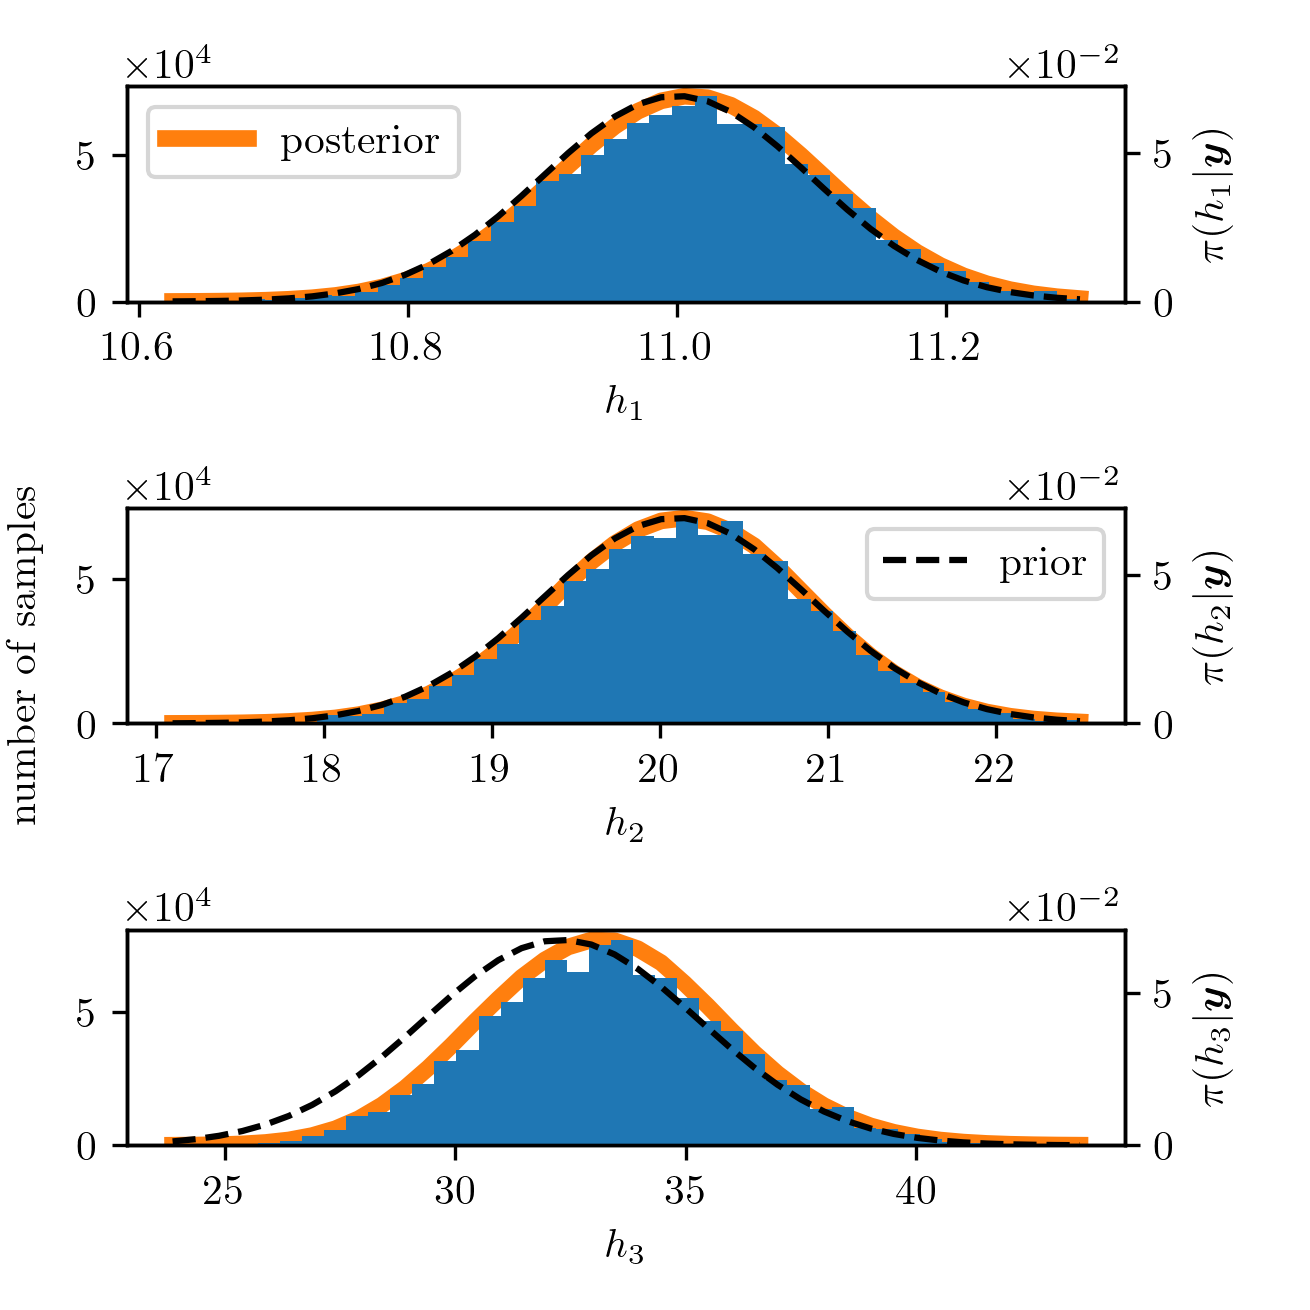
\includegraphics{PHdPTPost0.png}
	\caption[Histograms and TT approximation of posterior distribution as well as hyper-prior distribution.]{We plot the TT approximation of marginal posterior in orange and the samples as a histogram as well as the prior distribution with a dotted line.}
	\label{fig:PostHistTT0}
\end{figure}
\begin{figure}[ht!]
	\centering
	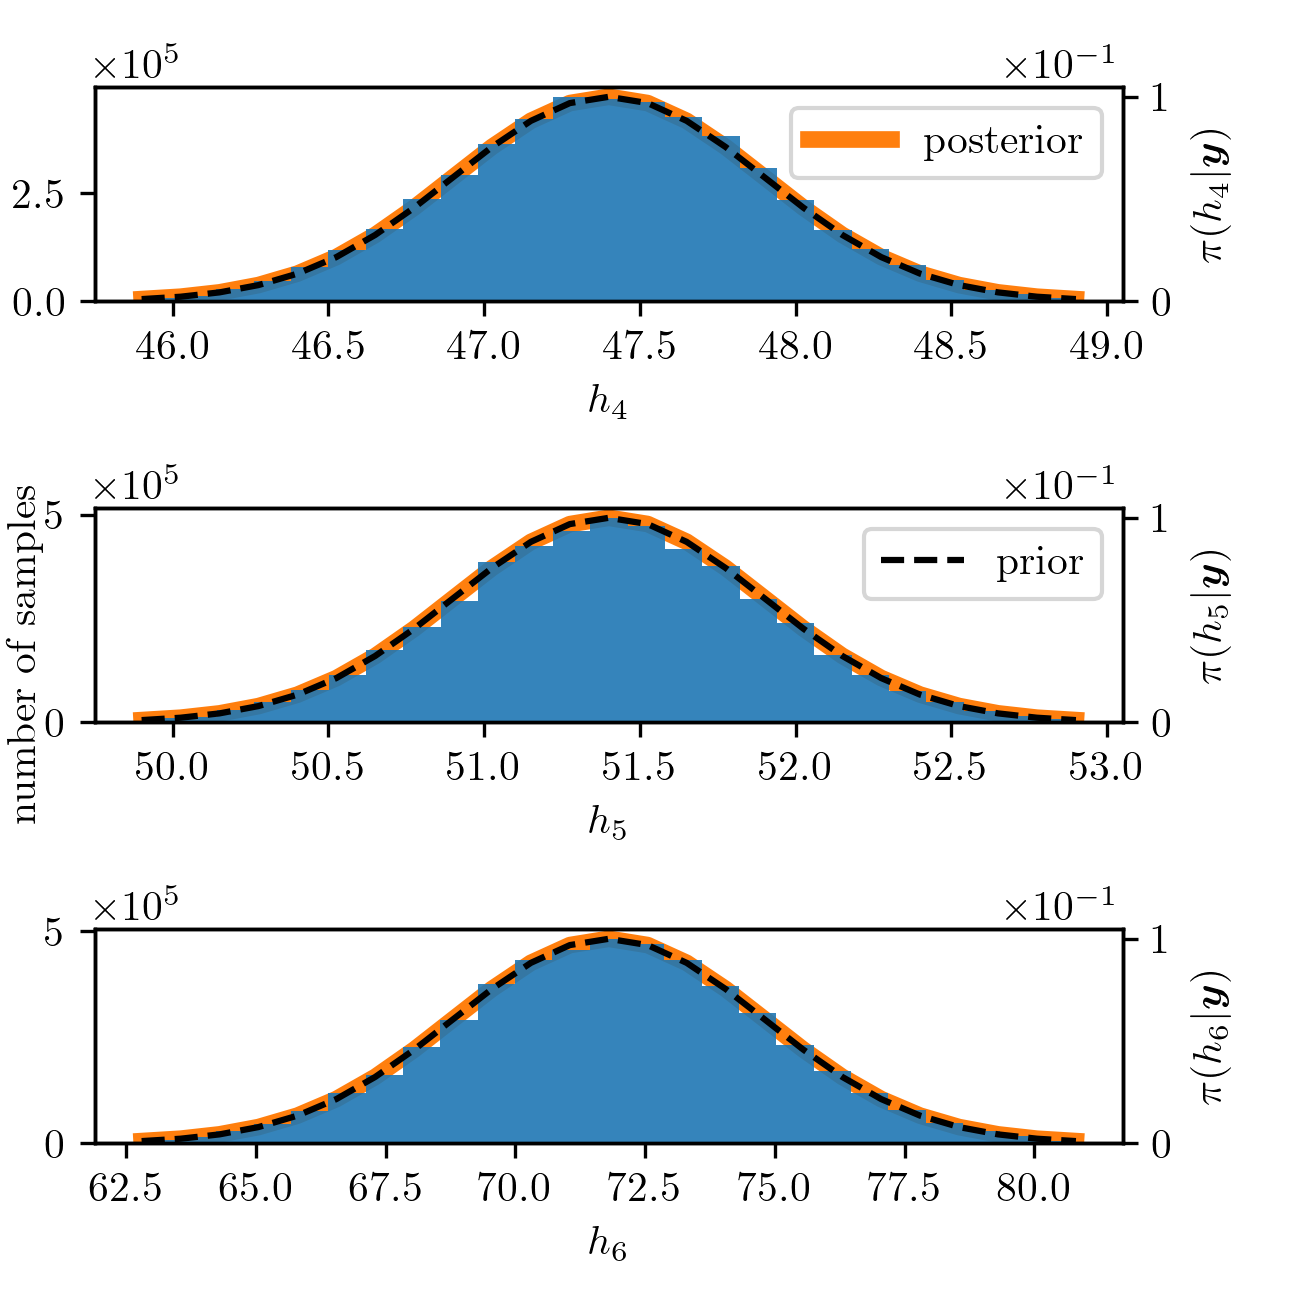
\includegraphics{PHdPTPost1.png}
	\caption[Histograms and TT approximation of posterior distribution as well as hyper-prior distribution.]{We plot the TT approximation of marginal posterior in orange and the samples as a histogram as well as the prior distribution with a dotted line.}
	\label{fig:PostHistTT1}
\end{figure}
\begin{figure}[ht!]
	\centering
	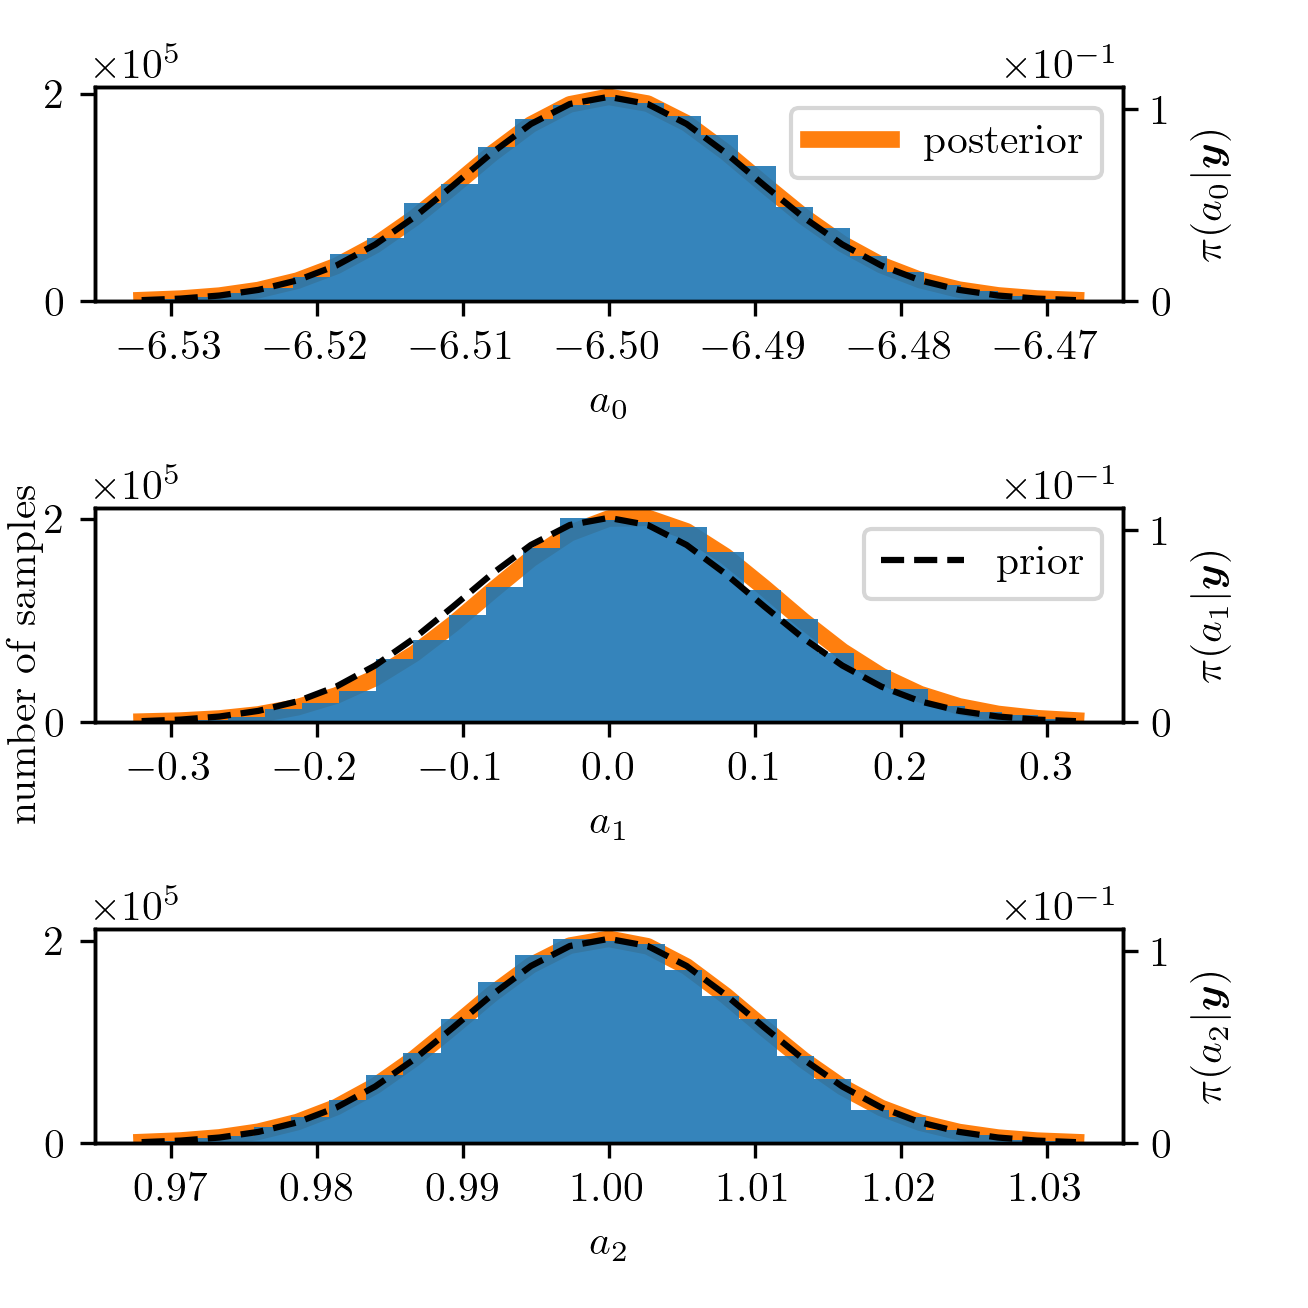
\includegraphics{PHdPTPost2.png}
	\caption[Histograms and TT approximation of posterior distribution as well as hyper-prior distribution.]{We plot the TT approximation of marginal posterior in orange and the samples as a histogram as well as the prior distribution with a dotted line.}
	\label{fig:PostHistTT2}
\end{figure}
\begin{figure}[ht!]
	\centering
	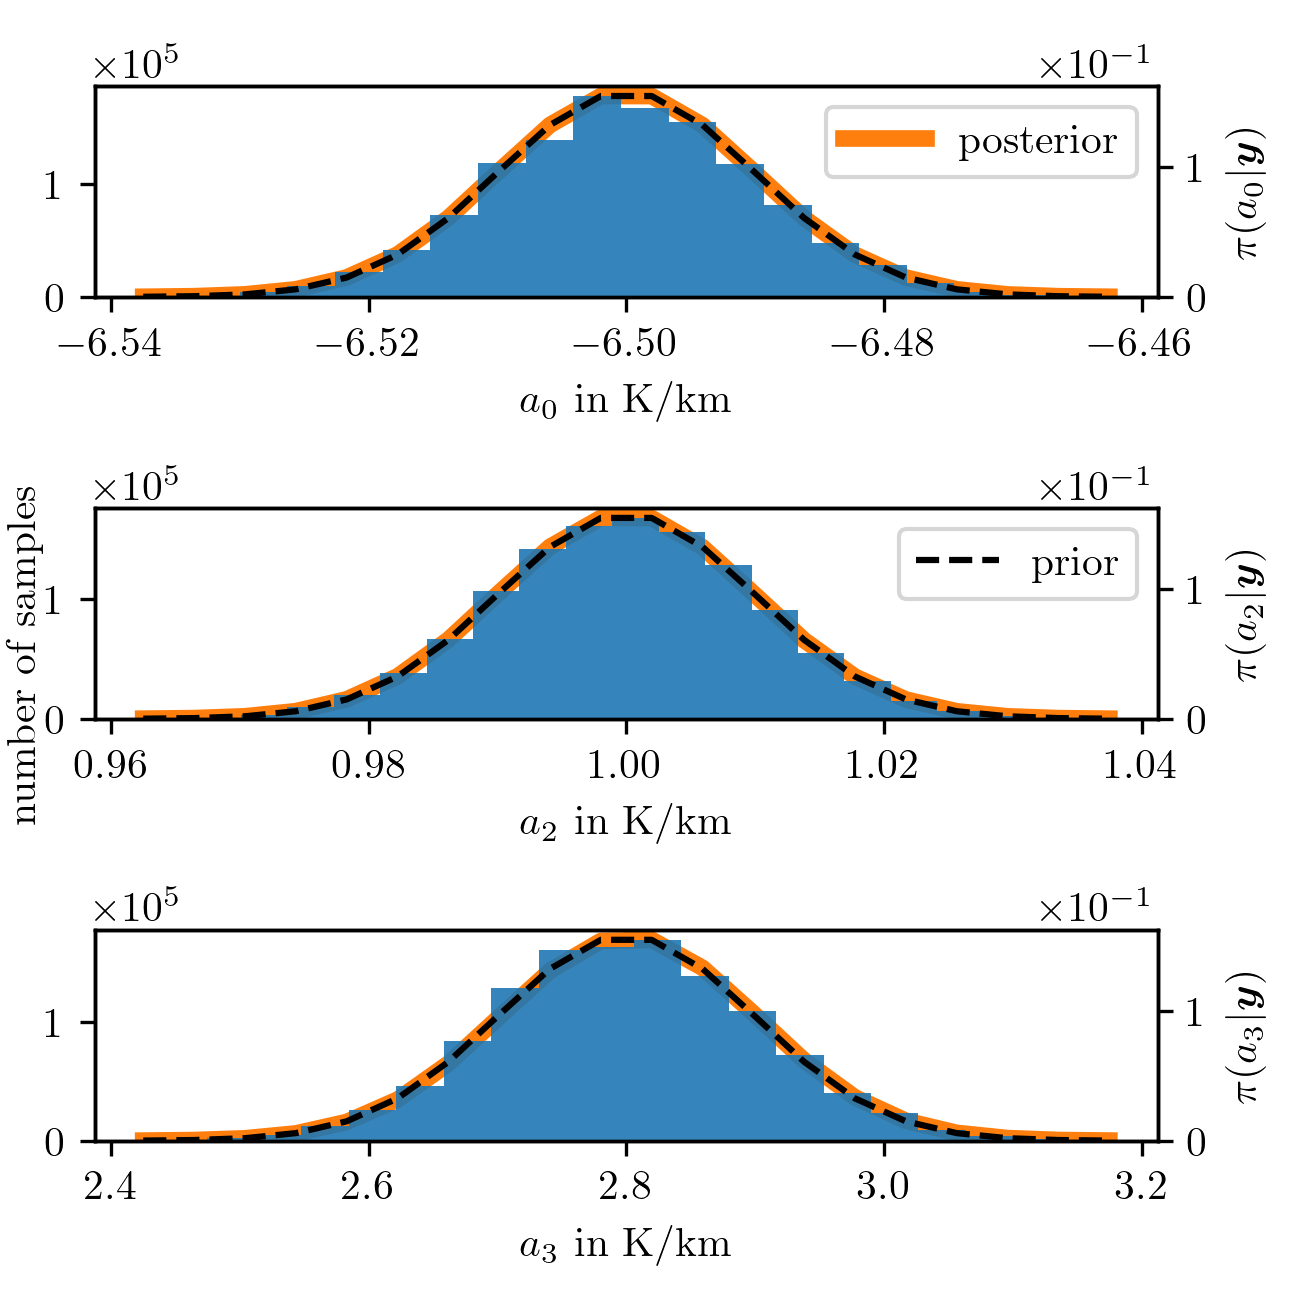
\includegraphics{PHdPTPost3.png}
	\caption[Histograms and TT approximation of posterior distribution as well as hyper-prior distribution.]{We plot the TT approximation of marginal posterior in orange and the samples as a histogram as well as the prior distribution with a dotted line.}
	\label{fig:PostHistTT3}
\end{figure}
\begin{figure}[ht!]
	\centering
	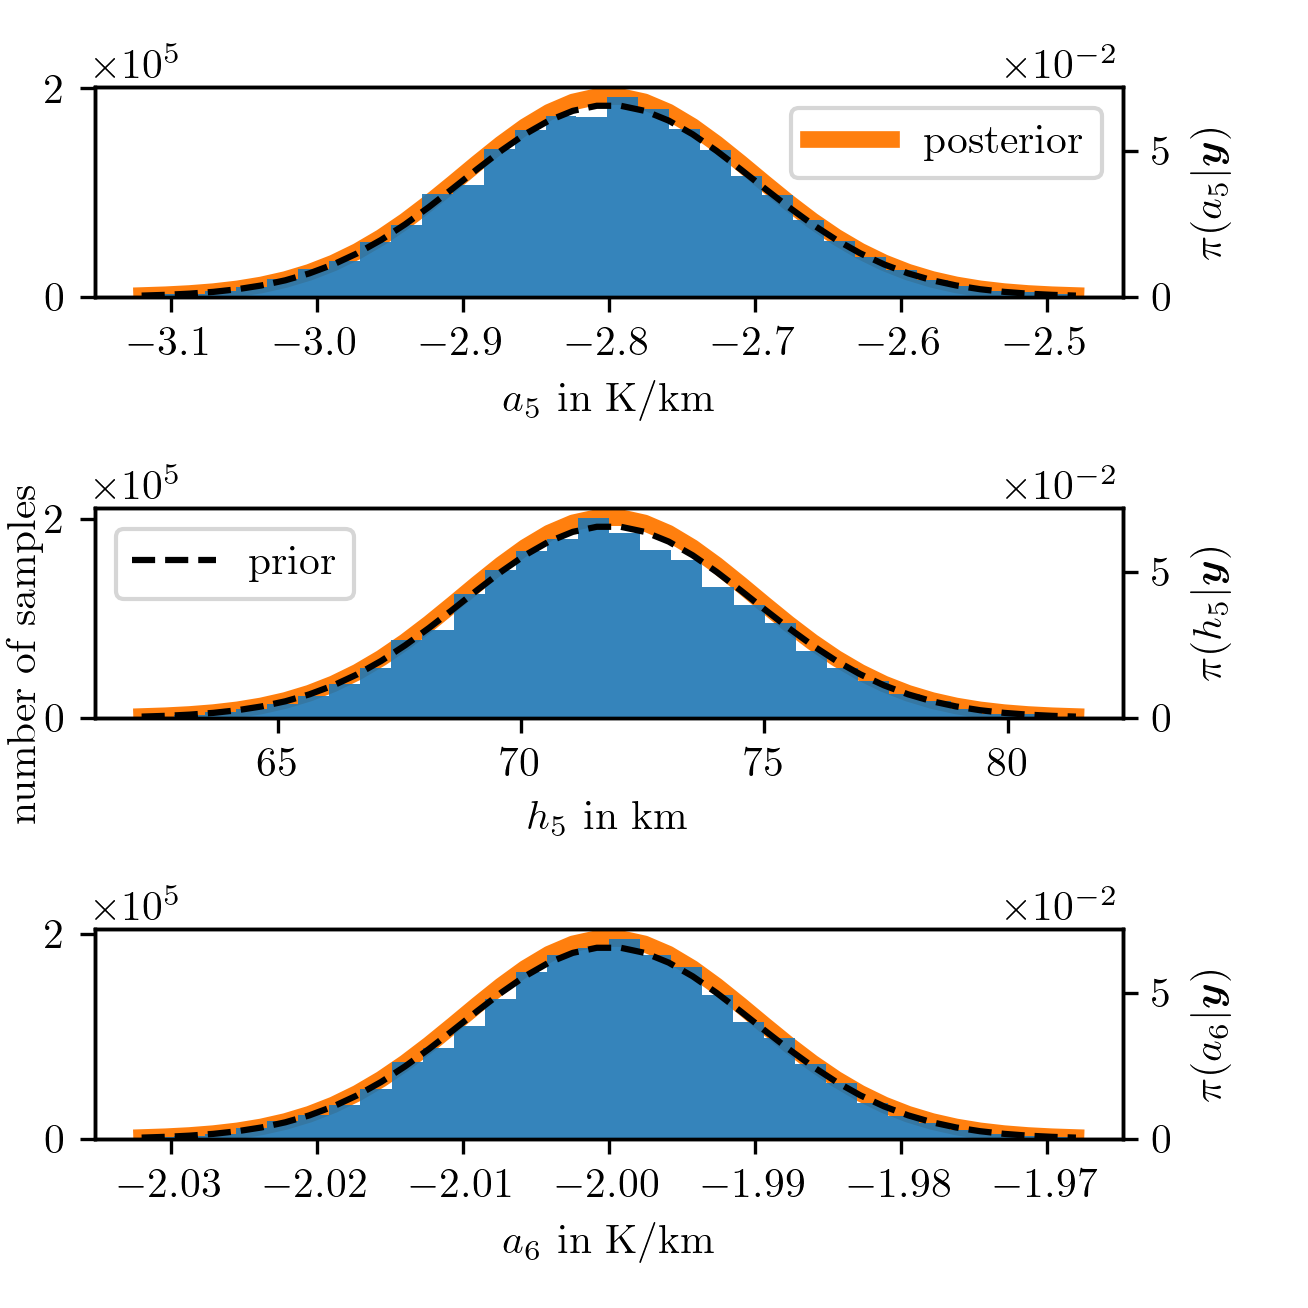
\includegraphics{PHdPTPost4.png}
	\caption[Histograms and TT approximation of posterior distribution as well as hyper-prior distribution.]{We plot the TT approximation of marginal posterior in orange and the samples as a histogram as well as the prior distribution with a dotted line.}
	\label{fig:PostHistTT4}
\end{figure}
We define a grid for each of the hyper-parameters, see Tab. \ref{tab:priors}, and set the grid points to $40$ and optimise over a set number of ranks equal to the dimension of 15.
To define the constant c we evaluate $\frac{\gamma}{2} \left\Vert \bm{y}- \bm{A} \frac{\bm{p}}{\bm{T}}  \right\Vert^2 + \ln{\pi(h_1,p_0,b_1,b_2,\bm{h_T},\bm{c_T},\bm{a_T})}$ at $100$ randomly chosen grid points and set $c$ to the negative half of the maximum value of those.
We terminate the \texttt{rect\_cross.cross} algorithm from the \texttt{ttpy} python package if the relative error provided by the algorithm is smaller than $0.1$ or after 10 sweeps, which takes roughly $1-2$ mins on a MacBook Pro from 2019 with 2.4 Ghz quadcore intel core i5 processor.
Then we calculate the marginals as in section \ref{sec:tensortrain} with a constant $= 1e-15$ and plot the results in Fig. \ref{fig:PostHistTT0} to \ref{fig:PostHistTT4} as an orange line.

On the same grid we run the t-walk, with the constant set to zero as the t-walk evaluates the function $- \ln{\pi(h_1,p_0,b_1,b_2,\bm{h_T},\bm{c_T},\bm{a_T} | \bm{y}, \gamma, \bm{x}) }$ we do not run into numerical issues.
We download the t-walk from \cite{christentwalkaccess} and let it take $1000000$ steps plus a burn-in period of $1000$, which takes around $7$ mins on the same laptop.
The resulting histogram are plotted in Fig. \ref{fig:PostHistTT0} to \ref{fig:PostHistTT4}, additionally we plot the trace of the samples in Fig. \ref{fig:TraceTwalk}
\textcolor{red}{integrated autocorrelation time, roughly efficient independent samples}
\clearpage

Resukts of TT and t-walk overlap say the same
for temperatuer we do not gain any more information than priors
Priors are posterior
For pressure the  gain more information
\textcolor{red}{grid size refer to figure}

Then we can either fit normal distribution to the marginals or draw samples from the output of the t-walk to calculate temperature and pressure profiles according to their respective functions, see Eq. \ref{eq:tempFunc} and \ref{eq:pressFunc}.
\begin{figure}[ht!]
	\centering
	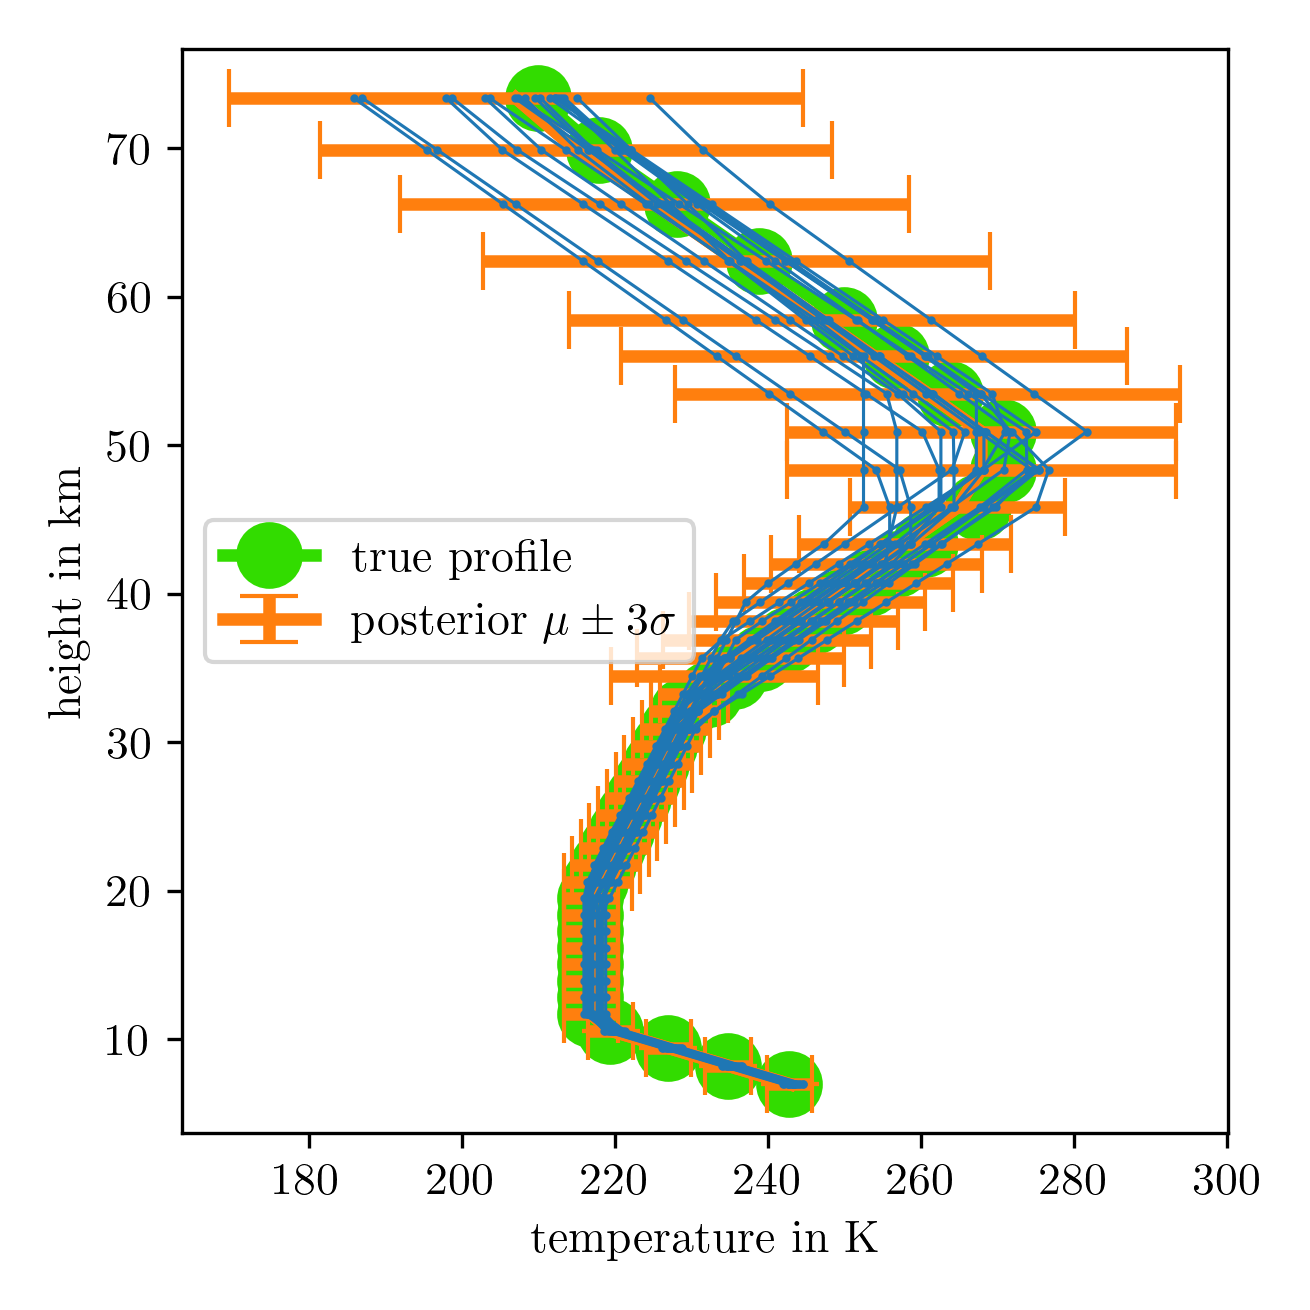
\includegraphics{TempPostMeanSigm.png} 
	\caption[Temperature posterior samples.]{We take samples from the posterior distribution, as plotted in Figures \ref{fig:PostHistTT0} to \ref{fig:PostHistTT3} and plot the corresponding temperature function, see Eq: \ref{eq:tempFunc}. }
	\label{fig:TempPost}
\end{figure}

\begin{figure}[ht!]
	\centering
	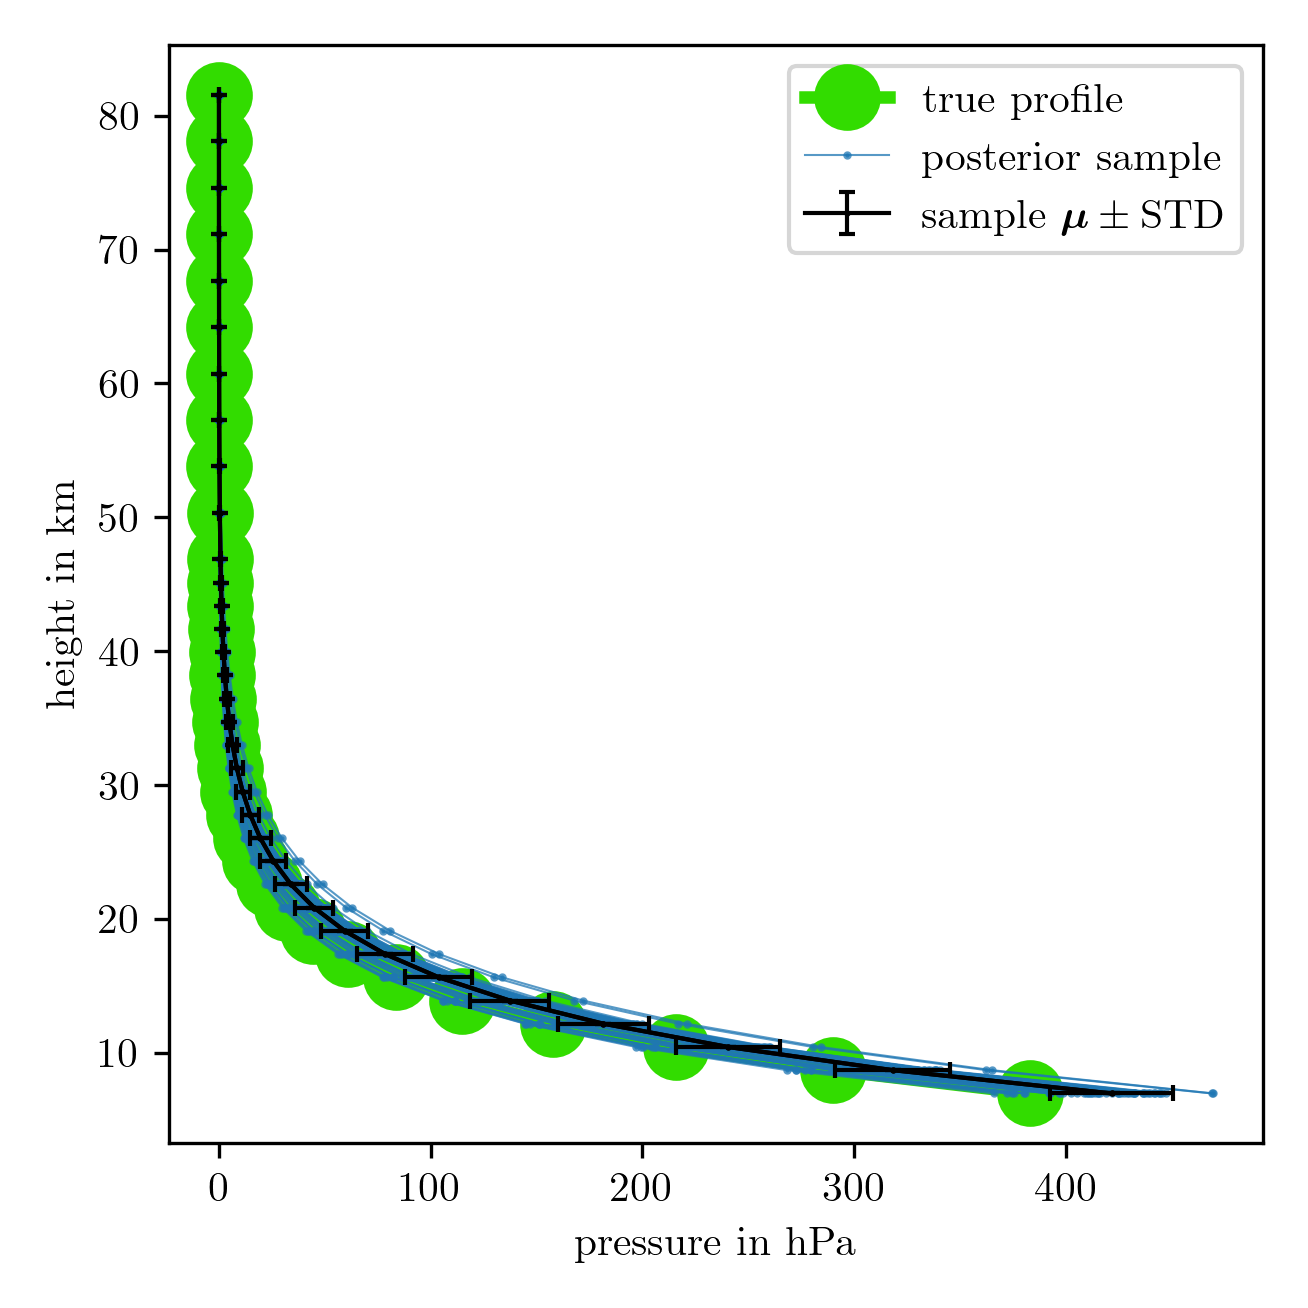
\includegraphics{PressPostMeanSigm.png}
	\caption[Pressure posterior samples.]{We take samples from the posterior distribution, as plotted in Fig. \ref{fig:PostHistTT4} and plot the corresponding pressure function, see Eq: \ref{eq:pressFunc}.}
	\label{fig:PressPost}
\end{figure}




